% KV-Mesh: a prototype for cache-affinity routing and tiered KV state
% management in distributed LLM serving.
%
% Build with:  tectonic kv-mesh.tex
% The generated tables and figures live in tables/ and figures/ and are
% produced by experiments/scripts/make_report.py.

\documentclass[10pt,twocolumn]{article}

\usepackage[letterpaper,margin=0.72in,columnsep=0.26in]{geometry}
\usepackage[T1]{fontenc}
\usepackage{textcomp}
\usepackage{mathptmx}
\usepackage{amsmath}
\usepackage{amssymb}
\usepackage{booktabs}
\usepackage{graphicx}
\usepackage{multirow}
\usepackage{array}
\usepackage{url}
\usepackage{xcolor}
\usepackage{listings}
\usepackage[hidelinks]{hyperref}

\definecolor{kvblue}{RGB}{23,54,93}
\definecolor{kvgray}{RGB}{110,110,110}

\lstset{
  basicstyle=\ttfamily\scriptsize,
  breaklines=true,
  frame=single,
  framerule=0.3pt,
  rulecolor=\color{kvgray},
  backgroundcolor=\color{gray!6},
  columns=fullflexible,
  showstringspaces=false,
  xleftmargin=1.5ex,
  xrightmargin=0ex,
  keywordstyle=\color{kvblue}\bfseries,
  commentstyle=\color{kvgray}\itshape,
}

\newcommand{\kvmesh}{\textsc{KV-Mesh}}
\newcommand{\hit}{\ensuremath{h(p)}}

\title{\kvmesh: A Prototype for Cache-Affinity Routing and Tiered\\
Key--Value State Management in Distributed LLM Serving}
\author{Ayaan Shaheer\\
Independent Researcher\\
{\small\url{https://github.com/AyaanShaheer/kv-mesh}}}
\date{}

\begin{document}
\maketitle

\begin{abstract}
Repeated prompts are common in multi-turn dialogue, retrieval-augmented
generation and agent workflows. When inference requests are dispatched without
regard to cache locality, a request may reach a worker that cannot reuse state
another worker has already computed, and the prefill work has to be redone.
This paper presents \kvmesh, a distributed-serving prototype that combines a
Go/gRPC routing gateway, Python worker processes, heartbeat-based worker-state
reporting, prompt-fingerprint routing, and a C++/pybind11 host-memory pool.
The gateway keeps a time-bounded worker registry and preferentially dispatches a
request to a live worker whose advertised cache index contains the request
fingerprint; otherwise it falls back to round-robin selection. The prototype
also models a two-tier cache lifecycle in which entries are evicted from a
small simulated fast tier into a host-memory byte pool and fetched back on
demand.

We report a complete, reproducible evaluation rather than a set of claims
without evidence. Three experimental arms are used: a discrete-event simulator
of the control plane, a live-system arm that drives the real Go gateway and
the real Python workers over gRPC, and microbenchmarks of the routing decision
and of the byte pool. Across a factorial sweep of 2{,}880 simulated
configurations, with five repetitions of 10{,}000 requests each, the affinity
policy keeps 6 to 10 percentage points more of the reusable state in the
fast tier than round-robin does when the working set exceeds the fast tier,
while the true cache-hit rate moves by less than one point because the host
tier absorbs most of the difference. The advantage vanishes entirely under a
low-reuse workload --- the regime in which the routing lookup is pure
overhead --- and the locality is bought with queueing delay, which grows by
two orders of magnitude for the affinity policy and by three for an oracle
policy between a lightly and a heavily loaded mesh. We
also quantify the price of staleness: a request routed on a stale
advertisement is served from a slower tier, and the fraction of such requests
grows with the heartbeat period and with heartbeat loss. The measured
routing decision costs 0.35--1.71\,$\mu$s for 1--128 registered workers in
the Go implementation, which is negligible beside any realistic prefill.

The contribution is not a new cache-aware routing algorithm; the paper states
plainly which prior art already covers that ground. It is an openly
inspectable prototype, a measurement framework that separates control-plane
routing behaviour from inference performance, and an evidence base for the
claim that mesh-level cache locality is useful only inside a specific regime,
with a specific cost.
\end{abstract}

\noindent\textbf{Keywords:} large language model serving; KV cache; prefix
caching; cache affinity; distributed routing; tiered memory; gRPC; systems
evaluation

\section{Introduction}

Autoregressive transformer inference processes an input prompt before
generating output tokens. The attention key/value (KV) state produced while
processing the prompt can be retained and reused when a later request shares a
compatible prefix, which avoids recomputing the corresponding prompt tokens.
Whether that reuse is possible depends on three things: whether the needed
state still exists, whether the cache identity used to look it up is valid,
and whether the request is actually sent to the node that holds it.

Prefix caching is already supported by production serving systems such as
vLLM~\cite{vllm_prefix_caching}, and research systems such as LMCache
explore broader storage, reuse and movement of KV state~\cite{lmcache}.
The problem considered here is narrower: when several independent workers serve
related requests, a gateway that ignores cache locality may send a request to a
worker that lacks reusable state even though another healthy worker holds it.

\kvmesh{} is an exploratory prototype for coordinating such workers. A Go
gateway tracks worker identifiers, addresses, heartbeat timestamps, cache
fingerprints and reported utilisation. A Python worker reports its state
through gRPC and exposes a streaming generation method. A C++ extension stores
byte payloads in a host-memory map and supplies offload/prefetch-shaped
operations. The design is deliberately small enough to inspect and extend,
which makes it suitable for a controlled systems experiment.

This paper does not claim that cache-aware routing, KV-cache reuse or
host-memory offloading is new in itself. It asks whether a lightweight mesh
control plane that combines cache-affinity routing with worker-liveness
metadata improves routing locality under constrained and changing worker
state, and what evidence is required to validate that claim against simple
baselines. The revision documented here answers that question with measurements
rather than with assertions: the previously empty results section is now
populated by an executed factorial sweep, a live-system arm that exercises the
real implementation, and microbenchmarks of the two components whose cost the
paper's claims depend on.

\subsection{Research questions}

\begin{itemize}
\item \textbf{RQ1}: Under repeated-prefix workloads, how does cache-affinity
routing change the cache-hit rate relative to round-robin routing?
\item \textbf{RQ2}: How do heartbeat period, metadata staleness and worker
churn affect routing accuracy and failed requests?
\item \textbf{RQ3}: What routing overhead does the gateway add as worker count
and request rate increase?
\item \textbf{RQ4}: When host-memory retrieval is modelled or implemented,
under which cache sizes and reuse distances is offload/prefetch preferable to
recomputation?
\end{itemize}

\subsection{Contributions}

\begin{itemize}
\item An open prototype architecture joining a Go/gRPC routing gateway with
Python workers and a pybind11/C++ byte-pool interface, with the routing
decision, the registry and the telemetry path instrumented so that every
decision can be audited after the fact.
\item A cache-affinity decision path that prefers live workers advertising a
matching request fingerprint and uses round-robin fallback on a reported miss,
made deterministic and free of the data race that the earlier revision
exhibited (Appendix~\ref{app:engineering}).
\item An experimental apparatus with three arms --- a simulator of the control
plane, a live-system arm against the real binaries, and component
microbenchmarks --- together with a protocol that separates control-plane
routing behaviour from model-inference performance.
\item A source-level limitation analysis that separates implemented code,
modelled behaviour and planned production integration, and an implementation
roadmap for moving from simulated state to genuine engine-managed KV tensors.
\end{itemize}

\section{Background and Related Work}

\subsection{KV caching and prefix reuse}

A transformer serving engine may preserve attention keys and values so that a
later request with a matching prefix avoids recomputing the corresponding
prompt tokens. vLLM documents automatic prefix caching using hashes over token
blocks and preceding-prefix context~\cite{vllm_prefix_caching}. A crucial
distinction for \kvmesh{} is that its fingerprint is computed over the entire
raw prompt string. This is not equivalent to token-block prefix matching: it
recognises exact string equality only, is sensitive to formatting and
tokenisation differences, and does not by itself establish that two requests
have a safely reusable token prefix. A production design should use an
engine-compatible cache key that includes the model and version, the
tokeniser, any relevant adapter, the cache format and the block/prefix
identity.

\subsection{KV-cache storage and transfer}

LMCache describes a cache layer that enables reuse and movement of KV state
across requests and engines, including tiered storage and transfer
mechanisms~\cite{lmcache}. Other work, including CacheGen, studies KV-cache
compression and streaming~\cite{cachegen}. These systems show that moving
cache state is an established research area. \kvmesh{}'s C++ component should
therefore be described precisely as a host-memory byte-pool prototype: it
copies an input byte string into a C++ vector and returns that byte string on
retrieval. The Python worker supplies a synthetic 1\,MiB payload when an entry
is evicted. The present code does not allocate CUDA memory, access a GPU
tensor, use pinned host memory, or perform a PCIe transfer. These are
implementation opportunities, not experimentally established features.

\subsection{Serving-system scheduling}

Serving research has studied workload-aware allocation and separation of prompt
prefill from token decoding. DistServe, for example, disaggregates these phases
to optimise serving goodput under latency constraints~\cite{distserve}.
\kvmesh{} addresses a different control point: it selects a worker based on
advertised cache state before forwarding a request. These approaches are
complementary in principle, but no integration or comparison with DistServe is
implemented in the current repository.

\section{System Design}

\subsection{Components and request path}

The system consists of (i) a Go gateway exposing gRPC services, (ii) Python
worker servers, (iii) a protocol-buffer interface for generation and heartbeat
reporting, and (iv) a C++ extension that keeps host-memory byte entries. A
client sends a generation request to the gateway. The gateway asks the router
for a worker, opens a gRPC client stream to that worker, and relays response
chunks to the client. Workers periodically submit a heartbeat with their ID,
reachable address, utilisation estimate, and the fingerprints currently
resident in the simulated fast tier.

Table~\ref{tab:components} maps each component to the code that implements it
and to the file that changed in this revision.

\begin{table}[t]
\centering
\caption{Components and their implementation.}
\label{tab:components}
\setlength{\tabcolsep}{3pt}
\begin{tabular}{p{0.21\columnwidth}p{0.36\columnwidth}p{0.25\columnwidth}}
\toprule
\textbf{Component} & \textbf{Current responsibility} & \textbf{Evidence in implementation} \\
\midrule
Go gateway & Receives heartbeat updates; selects worker; proxies the streamed response; emits a decision log and a metrics endpoint &
\texttt{gateway/\allowbreak main.go} \\
Routing table & Maintains worker records and their advertised fingerprints; rejects workers last seen 10\,s ago; maintains a deterministic, ID-sorted view of the live set &
\texttt{gateway/\allowbreak router/\allowbreak router.go} \\
Python worker & Reports every 3\,s; models two resident cache slots; yields fixed synthetic text chunks; records per-request ground truth &
\texttt{worker/\allowbreak main.py} \\
C++/pybind11 pool & Stores and returns byte vectors keyed by a 64-bit fingerprint; optionally bounded with FIFO eviction &
\texttt{worker/\allowbreak cpp\_extension/\allowbreak memory\_manager.cpp} \\
Protocol buffers & Define \texttt{GenerateStream}, \texttt{SendHeartbeat} and the telemetry fields used by the evaluation &
\texttt{proto/\allowbreak kvmesh.proto} \\
\bottomrule
\end{tabular}
\end{table}

\subsection{Cache-affinity routing policy}

Let $W(t)$ be the set of workers whose last heartbeat was observed within the
10-second liveness window. For request prompt $p$, the router computes a
64-bit fingerprint $h(p)$. If there exists an active worker $w$ whose
advertised set $C_w$ contains $h(p)$, the router selects the
least-loaded such worker, breaking ties by advertised fast-tier occupancy and
finally by worker identifier. Otherwise it selects a worker using a rotating
index over the ID-sorted active-worker slice. This is a membership-based
affinity policy, not a globally optimal scheduler: the code does not score
queue depth beyond a tie-break, estimated prefill cost, cache-entry size, or
the number of reusable prefix tokens.

Figure~\ref{fig:policy} gives the decision procedure as implemented.

\begin{figure}[t]
\centering
\fbox{\begin{minipage}{0.9\columnwidth}
\footnotesize\ttfamily
\setlength{\parskip}{2pt}
1.\ \ active $\leftarrow$ workers with heartbeat age $<$ TTL, sorted by ID\\
2.\ \ if active is empty: return "no active workers"\\
3.\ \ $h \leftarrow$ HashPrompt(prompt)\\
4.\ \ matches $\leftarrow\{w \in$ active$ : h \in C_w\}$\\
5.\ \ if matches is non-empty:\\
6.\ \ \ \ return argmin over matches of (queue\_depth, occupancy, ID)\\
7.\ \ $\leftarrow$ (cursor + 1) mod |active|\\
8.\ \ return active[$\vert$]
\end{minipage}}
\caption{The routing decision as implemented in \texttt{gateway/\allowbreak router/\allowbreak router.go}.}
\label{fig:policy}
\end{figure}

Two properties of this procedure are worth stating explicitly because the
earlier revision of this system violated both. First, the worker set is
visited in a \emph{stable} order, so a given registry state always yields the
same decision; the previous implementation iterated a Go map, which made
placement depend on randomised map iteration order. Second, the rotating index
is a single atomic counter rather than a field mutated under a read lock, so
concurrent requests cannot corrupt it.

\subsection{Cache identity and state}

The Go and Python hash helpers both take the first 16 hexadecimal digits of an
MD5 digest of the UTF-8 prompt string and parse them as an unsigned 64-bit
integer. Matching functions make the prototype interoperable, and the
experiment harness asserts this agreement at run time, but a 64-bit truncated
fingerprint carries collision risk and does not bind the key to model or
tokeniser identity. For a real implementation one should use a
collision-resistant cache key or verify full key material, and ensure that
cache residency comes from the inference engine rather than from a separately
maintained approximation.

\subsection{Tiered-memory prototype}

The worker models a two-slot fast tier as a Python list and applies FIFO
eviction. When it evicts an entry, it constructs a 1\,MiB byte string and
passes it to the C++ extension, which copies the bytes into a vector in an
unordered map. A prefetch retrieves and erases the saved bytes. This revision
adds an optional bound on the host pool, so that the host tier is a resource
that can be exhausted rather than an unbounded sink; the pool then evicts its
oldest entry. This tests the control-flow shape of offload and retrieval, but
not the bandwidth, synchronisation, correctness, fragmentation or latency of
GPU-to-CPU movement. The README's PCIe and GPU-VRAM descriptions should be
read as intended architecture rather than literal behaviour in the current
code.

\subsection{Liveness and telemetry}

Workers attempt to send heartbeats every three seconds, and the router
excludes a worker whose most recently received heartbeat is at least ten
seconds old. The gateway replaces the stored worker record on every heartbeat.
This revision adds a monotonic per-instance heartbeat sequence number and a
per-process instance identifier, so that out-of-order or duplicated heartbeats
are rejected while a worker that restarts under the same logical identifier is
still accepted. The gateway also reaps expired workers from the registry
periodically and exposes a JSON metrics endpoint.

\section{Implementation Status and Assumptions}

A research paper should distinguish implemented code, modelled behaviour and
planned production integration. Table~\ref{tab:status} makes that separation
explicit. The right-hand column states the strongest claim the evidence in
this paper supports.

\begin{table}[t]
\centering
\caption{Implementation status established by source inspection and by
measurement, with the claim each capability permits.}
\label{tab:status}
\setlength{\tabcolsep}{3pt}
\begin{tabular}{p{0.29\columnwidth}p{0.29\columnwidth}p{0.25\columnwidth}}
\toprule
\textbf{Capability} & \textbf{Status established by source inspection} & \textbf{Claim permitted in this paper} \\
\midrule
Multi-worker gRPC gateway and streaming relay & Implemented in Go; workers expose a gRPC stream & The prototype relays streamed output over real gRPC; measured end to end \\
Heartbeat registry and TTL filtering & Implemented in Go/Python at a 3\,s heartbeat and 10\,s expiry window; out-of-order heartbeats rejected & Liveness metadata and expiry behaviour can be studied, and were \\
Exact-prompt fingerprint affinity & Implemented using truncated MD5-derived 64-bit fingerprints and advertised resident entries & Placement behaviour for exact prompt repeats can be evaluated \\
Round-robin and least-loaded fallback & Implemented as selectable policies & Routing decisions can be compared against simple baselines \\
Deterministic placement and race-free cursor & Implemented; verified by unit tests and the race detector & Placement is reproducible and the routing path is free of the earlier data race \\
Real model inference & Not established; the worker yields fixed synthetic text chunks & No real-model TTFT, throughput or output-quality claim is made \\
Real GPU KV tensor cache & Not implemented in the inspected worker & No claim that cache reuse skips transformer prefill \\
GPU-to-CPU PCIe transfer & Not implemented; byte strings are copied to C++ host memory & Described as a simulated byte-pool offload/prefetch \\
Dynamic VRAM usage & The reported value is list length divided by the simulated capacity & Called a simulated occupancy indicator, not actual VRAM telemetry \\
\bottomrule
\end{tabular}
\end{table}

\section{Evaluation Methodology}

This section specifies the experiment. The results in
Section~\ref{sec:results} were produced by executing it; the scripts, the
raw per-request records and the analysis code are listed in
Appendix~\ref{app:repro}.

\subsection{Experimental arms}

Three arms are used, each answering a different part of the evaluation.

\paragraph{Simulator arm (control plane).} A discrete-event simulator of the
mesh reproduces the gateway's routing logic in Python: worker-ID ordering, the
TTL liveness window, snapshot semantics for heartbeats, the atomic rotating
cursor, and a FIFO two-tier cache lifecycle with a bounded fast tier and an
optionally bounded host tier. It additionally models a FIFO server with a
constant service time, so that queueing delay and the least-loaded baseline
are meaningful, and it maintains ground truth about which tier actually holds
each entry. This arm carries the factorial sweep, because a live cluster
cannot be swept over hundreds of configurations.

\paragraph{Live-system arm (implementation).} The real Go gateway binary and
the real Python worker processes are started on the loopback interface and
driven over gRPC with a seeded request trace. The gateway records every
routing decision to a JSON Lines log together with its own decision latency;
the workers record the ground-truth cache status of every request they serve.
Correlating the two logs by request identifier yields the advertised-hit and
true-hit rates of the actual implementation, and the gateway's own timing
gives the routing overhead of the real code path. The simulator arm and the
live arm are reported separately and never pooled.

\paragraph{Microbenchmark arm (components).} The routing decision is
benchmarked in the Go implementation with \texttt{go test -bench}, and the
C++ byte pool is benchmarked through its pybind11 interface.

\subsection{Baselines}

\begin{itemize}
\item \textbf{Round-robin}: route each request to the next live worker without
examining cache state.
\item \textbf{Least-loaded}: route to the live worker reporting the lowest
queue depth. Where only occupancy is available, occupancy is used and is
explicitly not queue depth.
\item \textbf{Cache-affinity (\kvmesh)}: use a valid cache match first;
otherwise use the round-robin fallback.
\item \textbf{Oracle}: choose a worker that truly holds the entry according to
the simulator's ground truth. This is an upper bound on the affinity policy
and is not a deployable baseline.
\end{itemize}

\subsection{Workloads}

Table~\ref{tab:workloads} lists the workload constructions, the question each
one isolates and the primary metric.

\begin{table}[t]
\centering
\caption{Workload constructions.}
\label{tab:workloads}
\setlength{\tabcolsep}{3pt}
\begin{tabular}{p{0.19\columnwidth}p{0.33\columnwidth}p{0.29\columnwidth}}
\toprule
\textbf{Workload} & \textbf{Construction and purpose} & \textbf{Primary metric} \\
\midrule
Exact repeats & Replay a small key space repeatedly, with Poisson inter-arrival times. Tests exact-key locality. & Affinity hit rate; routing overhead \\
Hot set / Zipf & Draw prompts from a skewed set where a small hot subset repeats often. Approximates recurring system prompts and shared context identifiers. & Hit rate; request completion rate \\
Uniform / low reuse & Choose prompt identifiers uniformly from a large key space. Tests the affinity benefit when reuse is low. & Overhead; load distribution \\
Worker churn & Terminate and restart workers during the replay. Tests stale registrations and failure recovery. & Routing errors; recovery behaviour \\
Heartbeat delay / loss & Inject heartbeat delay, drop and jitter. Measures the effect of stale cache state. & False-affinity rate; degraded-locality rate \\
Capacity pressure & Vary fast-tier slots, host-tier slots and reuse distance. Exercises the eviction and byte-pool path. & Tier hit rate; copied bytes; operation latency \\
\bottomrule
\end{tabular}
\end{table}

\subsection{Experimental factors and repetitions}

The main sweep crosses four factors: worker count in $\{1,2,4,8\}$, fast-tier
capacity in $\{2,8,32,128\}$ entries, heartbeat interval in $\{1,3,5\}$\,s,
and the staleness window fixed at 10\,s; with four policies, three workloads
and five repetitions of 10{,}000 requests this yields 2{,}880 simulated runs.
Each repetition replays a \emph{different} trace, drawn from a distinct
workload seed, so that the replicates are independent samples rather than
replays of one trace. The offered load is expressed as a target utilisation per
worker, $\rho$, and the arrival rate is derived as
$\lambda = \rho W / s$ with $s = 5$\,ms of simulated service time; holding
$\rho$ fixed keeps the comparison between one and eight workers attributable
to the policy rather than to a difference in load. Scenario sweeps vary one
further factor at a time: the staleness window in $\{5,10,20\}$\,s, heartbeat
delay in $\{0,1,3\}$\,s, heartbeat jitter in $\{0,1\}$\,s, heartbeat loss in
$\{0,0.1,0.3\}$, churn interval in $\{5,15,30\}$\,s with downtime in
$\{0,5\}$\,s, fast-tier capacity in $\{2,\dots,128\}$, host-tier capacity in
$\{0,8,32,64,128,512\}$ entries, and offered load
$\rho \in \{0.25,0.5,0.75,0.9,1.05\}$.

\subsection{Metrics and definitions}

\begin{itemize}
\item \textbf{Routing cache-hit rate} = requests routed to a worker
advertising a matching key / total eligible requests.
\item \textbf{True cache-hit rate} = requests whose selected worker actually
retained the reusable state at execution time, verified from ground truth.
Reported separately from the advertised-hit rate.
\item \textbf{Stale-affinity rate} = requests routed on a matching
advertisement whose state was absent from both tiers at execution time,
divided by advertised-hit requests.
\item \textbf{Degraded-locality rate} = requests routed on a matching
advertisement whose state had been evicted from the fast tier and therefore
had to be fetched from the host tier, divided by advertised-hit requests.
This is the price of a stale advertisement: the request is still served, but
from a slower tier.
\item \textbf{Request failure rate} = failed or timed-out requests / submitted
requests.
\item \textbf{Worker imbalance} = coefficient of variation of the number of
requests assigned per worker.
\item \textbf{Routing overhead} = the gateway's decision time, measured by the
gateway itself in the live arm and by \texttt{go test -bench} in the
microbenchmark arm.
\item \textbf{Memory path latency} = measured time for store and retrieval in
the byte-pool microbenchmark. This is a host-memory copy latency and is never
labelled as a PCIe or GPU-transfer latency.
\end{itemize}

\subsection{Statistical analysis}

For every table cell the reported value is the mean over the repetitions of
that cell, with a 95\,\% bootstrap confidence interval obtained by
resampling the replicates (10{,}000 resamples). Policy comparisons use a
\emph{paired} bootstrap over the replicate index, together with Cohen's
$d$, because the same configuration is replayed under each policy and the
replicates are matched by repetition. Raw per-request records are archived for
the configurations that back the principal tables; the aggregate metrics of
every run are archived in full.

\subsection{Threats to the validity of the simulator}

The simulator is a model, not the system. Four properties are checked rather
than assumed. \emph{Faithfulness of the decision rule} is established by
construction: the simulator reimplements the Go router's ordering, liveness
and tie-break rules, and the routing path is additionally exercised against
the real binary in the live arm. \emph{Ground truth} is maintained by the
simulator itself, which records the tier in which each entry physically
resides, so that the advertised-hit and true-hit rates are measured rather
than inferred. \emph{Service time} is a constant; real prefill cost depends
on prompt length and on the engine, so the queueing results characterise the
\emph{policy's} behaviour under a queueing model and not any absolute
latency. \emph{The host tier is bounded} in the simulator, whereas the
prototype's byte pool is unbounded unless explicitly configured; the
unbounded configuration is included in the capacity sweep so that the effect
of this modelling choice is visible.

\section{Results}
\label{sec:results}

\subsection{Policy comparison at the reference configuration}

Table~\ref{tab:policy-comparison} compares the four policies at the
reference configuration (four workers, a fast tier of eight entries, a 3\,s
heartbeat and a 10\,s staleness window), and
Table~\ref{tab:significance} reports the paired bootstrap comparison against
round-robin.

\begin{table*}[t]
\centering
\scriptsize
\setlength{\tabcolsep}{2.5pt}
\caption{Policy comparison at the reference configuration (4 workers, fast tier of 8 entries, 3 s heartbeat, 10 s TTL). Brackets give bootstrap 95\% confidence intervals over 5 repetitions of 10,000 requests each. ``Stale'' is the fraction of advertised hits whose state was absent from both tiers at execution time; ``Degraded'' is the fraction that had to be served from the host tier instead of the fast tier. A dash means the quantity is undefined because the policy produced no advertised hits.}
\label{tab:policy-comparison}
\begin{tabular}{lcccccccccc}
\toprule
Workload & Policy & Adv. hit & True hit & Fast tier & Host tier & Stale & Degraded & CV & Fail \\
\midrule
Exact repeats & affinity & 37.6 \tiny [36.88, 38.26] & 97.4 \tiny [97.44, 97.44] & 22.6 \tiny [22.18, 23.00] & 74.9 \tiny [74.44, 75.26] & 0.0 \tiny [0.00, 0.00] & 61.9 \tiny [61.13, 62.54] & 0.0 \tiny [0.01, 0.02] & 0.0 \tiny [0.00, 0.00] \\
Exact repeats & round-robin & 0.0 \tiny [0.00, 0.00] & 97.4 \tiny [97.44, 97.44] & 12.2 \tiny [12.09, 12.34] & 85.2 \tiny [85.10, 85.35] & -- \tiny [--, --] & -- \tiny [--, --] & 0.0 \tiny [0.00, 0.00] & 0.0 \tiny [0.00, 0.00] \\
Exact repeats & least-loaded & 0.0 \tiny [0.00, 0.00] & 97.4 \tiny [97.44, 97.44] & 12.2 \tiny [11.89, 12.48] & 85.3 \tiny [84.96, 85.55] & -- \tiny [--, --] & -- \tiny [--, --] & 0.3 \tiny [0.34, 0.34] & 0.0 \tiny [0.00, 0.00] \\
Exact repeats & oracle & 0.0 \tiny [0.00, 0.00] & 99.4 \tiny [99.36, 99.36] & 49.6 \tiny [49.38, 49.93] & 49.7 \tiny [49.43, 49.98] & -- \tiny [--, --] & -- \tiny [--, --] & 0.0 \tiny [0.00, 0.00] & 0.0 \tiny [0.00, 0.00] \\
Hot set (Zipf) & affinity & 68.7 \tiny [68.34, 69.08] & 88.8 \tiny [88.77, 88.80] & 69.3 \tiny [68.75, 69.88] & 19.5 \tiny [18.89, 20.04] & 0.0 \tiny [0.00, 0.00] & 13.0 \tiny [12.56, 13.45] & 0.3 \tiny [0.25, 0.35] & 0.0 \tiny [0.00, 0.00] \\
Hot set (Zipf) & round-robin & 0.0 \tiny [0.00, 0.00] & 88.2 \tiny [87.95, 88.42] & 62.9 \tiny [62.72, 63.07] & 25.3 \tiny [25.01, 25.55] & -- \tiny [--, --] & -- \tiny [--, --] & 0.0 \tiny [0.00, 0.00] & 0.0 \tiny [0.00, 0.00] \\
Hot set (Zipf) & least-loaded & 0.0 \tiny [0.00, 0.00] & 88.2 \tiny [87.99, 88.37] & 62.9 \tiny [62.62, 63.12] & 25.3 \tiny [24.99, 25.70] & -- \tiny [--, --] & -- \tiny [--, --] & 0.3 \tiny [0.34, 0.35] & 0.0 \tiny [0.00, 0.00] \\
Hot set (Zipf) & oracle & 0.0 \tiny [0.00, 0.00] & 97.5 \tiny [97.49, 97.53] & 78.5 \tiny [78.20, 78.90] & 19.0 \tiny [18.62, 19.31] & -- \tiny [--, --] & -- \tiny [--, --] & 1.0 \tiny [0.89, 1.10] & 0.0 \tiny [0.00, 0.00] \\
Uniform (low reuse) & affinity & 0.7 \tiny [0.70, 0.76] & 2.0 \tiny [1.85, 2.06] & 0.3 \tiny [0.23, 0.27] & 1.7 \tiny [1.62, 1.79] & 67.8 \tiny [66.47, 69.10] & 31.1 \tiny [29.59, 32.69] & 0.0 \tiny [0.00, 0.00] & 0.0 \tiny [0.00, 0.00] \\
Uniform (low reuse) & round-robin & 0.0 \tiny [0.00, 0.00] & 1.8 \tiny [1.67, 1.86] & 0.2 \tiny [0.21, 0.24] & 1.5 \tiny [1.46, 1.63] & -- \tiny [--, --] & -- \tiny [--, --] & 0.0 \tiny [0.00, 0.00] & 0.0 \tiny [0.00, 0.00] \\
Uniform (low reuse) & least-loaded & 0.0 \tiny [0.00, 0.00] & 1.8 \tiny [1.77, 1.88] & 0.2 \tiny [0.21, 0.29] & 1.6 \tiny [1.55, 1.62] & -- \tiny [--, --] & -- \tiny [--, --] & 0.3 \tiny [0.34, 0.35] & 0.0 \tiny [0.00, 0.00] \\
Uniform (low reuse) & oracle & 0.0 \tiny [0.00, 0.00] & 7.1 \tiny [6.87, 7.25] & 0.8 \tiny [0.81, 0.88] & 6.2 \tiny [6.01, 6.43] & -- \tiny [--, --] & -- \tiny [--, --] & 0.0 \tiny [0.00, 0.01] & 0.0 \tiny [0.00, 0.00] \\
\bottomrule
\end{tabular}
\end{table*}


\begin{table}[t]
\centering
\scriptsize
\setlength{\tabcolsep}{2.5pt}
\caption{Paired bootstrap comparison of each policy against round-robin at the reference configuration. Differences are reported as fractions, so a difference of 0.064 is 6.4 percentage points. A dash in the Cohen's $d$ column means the effect is perfectly separated but its standardised size is undefined because the replicates had zero between-run variance.}
\label{tab:significance}
\begin{tabular}{lcccccccccc}
\toprule
Workload & Metric & Policy & Baseline & n & Diff & 95\% CI low & 95\% CI high & P(diff>0) & Cohen's $d$ \\
\midrule
Exact repeats & true\_hit\_rate & affinity & round-robin & 5 & 0.0000 & 0.0000 & 0.0000 & 0.0000 & -- \\
Exact repeats & true\_hit\_rate & least-loaded & round-robin & 5 & 0.0000 & 0.0000 & 0.0000 & 0.0000 & -- \\
Exact repeats & true\_hit\_rate & oracle & round-robin & 5 & 0.0192 & 0.0192 & 0.0192 & 1.0000 & -- \\
Exact repeats & fast\_tier\_hit\_rate & affinity & round-robin & 5 & 0.1032 & 0.0996 & 0.1074 & 1.0000 & 26.7939 \\
Exact repeats & fast\_tier\_hit\_rate & least-loaded & round-robin & 5 & -0.0004 & -0.0032 & 0.0026 & 0.3823 & -0.1470 \\
Exact repeats & fast\_tier\_hit\_rate & oracle & round-robin & 5 & 0.3739 & 0.3711 & 0.3772 & 1.0000 & 131.6995 \\
Hot set (Zipf) & true\_hit\_rate & affinity & round-robin & 5 & 0.0062 & 0.0035 & 0.0083 & 1.0000 & 2.8627 \\
Hot set (Zipf) & true\_hit\_rate & least-loaded & round-robin & 5 & 0.0002 & -0.0015 & 0.0020 & 0.5845 & 0.0861 \\
Hot set (Zipf) & true\_hit\_rate & oracle & round-robin & 5 & 0.0935 & 0.0910 & 0.0956 & 1.0000 & 42.9689 \\
Hot set (Zipf) & fast\_tier\_hit\_rate & affinity & round-robin & 5 & 0.0642 & 0.0582 & 0.0702 & 1.0000 & 12.1589 \\
Hot set (Zipf) & fast\_tier\_hit\_rate & least-loaded & round-robin & 5 & -0.0003 & -0.0012 & 0.0005 & 0.2509 & -0.1068 \\
Hot set (Zipf) & fast\_tier\_hit\_rate & oracle & round-robin & 5 & 0.1565 & 0.1539 & 0.1594 & 1.0000 & 43.1046 \\
Uniform (low reuse) & true\_hit\_rate & affinity & round-robin & 5 & 0.0019 & 0.0002 & 0.0030 & 0.9929 & 1.4972 \\
Uniform (low reuse) & true\_hit\_rate & least-loaded & round-robin & 5 & 0.0006 & -0.0008 & 0.0017 & 0.8333 & 0.6490 \\
Uniform (low reuse) & true\_hit\_rate & oracle & round-robin & 5 & 0.0531 & 0.0518 & 0.0544 & 1.0000 & 27.4562 \\
Uniform (low reuse) & fast\_tier\_hit\_rate & affinity & round-robin & 5 & 0.0003 & 0.0001 & 0.0004 & 1.0000 & 1.0400 \\
Uniform (low reuse) & fast\_tier\_hit\_rate & least-loaded & round-robin & 5 & 0.0002 & -0.0002 & 0.0006 & 0.8386 & 0.5072 \\
Uniform (low reuse) & fast\_tier\_hit\_rate & oracle & round-robin & 5 & 0.0062 & 0.0058 & 0.0067 & 1.0000 & 16.0600 \\
\bottomrule
\end{tabular}
\end{table}


The pattern is consistent across the three workloads and matches the
mechanism the policy is supposed to exploit. Under the exact-repeat workload
the affinity policy raises the fast-tier hit rate from 12.2\,\% to 22.6\,\%,
a paired difference of 10.3 percentage points with a 95\,\% interval of
[9.96, 10.74] and a bootstrap probability of 1.0 that the difference is
positive. Under the hot-set workload the corresponding difference is 6.4
points [5.82, 7.02]. The true-hit rate moves much less --- by 0.6 points
under the hot set --- because the host tier absorbs most of the difference:
an entry that is not in the fast tier can still be recovered from the host
tier without recomputation. The affinity policy therefore mostly changes
\emph{which tier} a hit is served from, and that is exactly the quantity the
round-robin baseline cannot influence.

The oracle row bounds what any cache-aware policy could have achieved in the
same runs. Under the hot set it reaches a 78.5\,\% fast-tier hit rate against
the affinity policy's 69.3\,\%. Over the round-robin baseline's 62.9\,\%
that leaves 15.6 points available, of which the membership rule captures 6.4
--- roughly two fifths --- and leaves the remainder as headroom for a policy
that reasons about reuse distance and queueing. The
least-loaded baseline is statistically indistinguishable from round-robin on
both metrics (differences of $+0.02$ and $-0.04$ points, with bootstrap
probabilities of 0.58 and 0.25 that the difference is positive): in this
workload, where the queueing delay is small, load balancing on its own
changes nothing.

The uniform workload is the important negative case. When the key space is
large relative to the trace, almost nothing is reusable: the affinity policy
reaches a 2.0\,\% true-hit rate against round-robin's 1.8\,\%, and the
oracle's 7.1\,\% shows that even a perfect placement policy has little to
work with. Worse, 67.8\,\% of the affinity policy's advertised hits were
\emph{stale} --- the worker advertised a fingerprint that was no longer in
either tier --- because a small advertised-hit count on a large key space is
mostly noise. Reporting this case is what makes the positive results
interpretable: locality is a bet that the next request will reuse what is
already resident, and the bet pays only when it is a good one.

\subsection{Worker count}

\begin{table*}[t]
\centering
\scriptsize
\setlength{\tabcolsep}{2.5pt}
\caption{Effect of the mesh size on cache locality under the hot-set workload (fast tier of 8 entries, 3 s heartbeat, 10 s TTL). The offered load is held at a constant utilisation per worker.}
\label{tab:worker-scaling}
\begin{tabular}{lccccccc}
\toprule
Workers & Policy & Adv. hit \% & True hit \% & Fast-tier \% & CV & p95 queue (ms) \\
\midrule
1 & affinity & 60.212 \tiny [56.0740, 63.9480] & 88.986 \tiny [88.9180, 89.0540] & 62.896 \tiny [62.5520, 63.3020] & 0.000 \tiny [0.0000, 0.0000] & 10.010 \tiny [9.6226, 10.3409] \\
1 & round-robin & 0.000 \tiny [0.0000, 0.0000] & 88.986 \tiny [88.9180, 89.0540] & 62.896 \tiny [62.5520, 63.3020] & 0.000 \tiny [0.0000, 0.0000] & 10.010 \tiny [9.6226, 10.3409] \\
1 & least-loaded & 0.000 \tiny [0.0000, 0.0000] & 88.986 \tiny [88.9180, 89.0540] & 62.896 \tiny [62.5520, 63.3020] & 0.000 \tiny [0.0000, 0.0000] & 10.010 \tiny [9.6226, 10.3409] \\
1 & oracle & 0.000 \tiny [0.0000, 0.0000] & 88.986 \tiny [88.9180, 89.0540] & 62.896 \tiny [62.5520, 63.3020] & 0.000 \tiny [0.0000, 0.0000] & 10.010 \tiny [9.6226, 10.3409] \\
2 & affinity & 65.510 \tiny [62.8920, 68.2480] & 88.978 \tiny [88.7620, 89.1720] & 66.856 \tiny [66.1780, 67.6780] & 0.256 \tiny [0.1923, 0.3125] & 15.336 \tiny [14.2722, 16.3995] \\
2 & round-robin & 0.000 \tiny [0.0000, 0.0000] & 88.628 \tiny [88.4740, 88.8220] & 62.972 \tiny [62.5720, 63.4100] & 0.000 \tiny [0.0000, 0.0000] & 4.442 \tiny [4.2947, 4.5860] \\
2 & least-loaded & 0.000 \tiny [0.0000, 0.0000] & 88.650 \tiny [88.5000, 88.8260] & 62.908 \tiny [62.6220, 63.2060] & 0.236 \tiny [0.2333, 0.2385] & 4.766 \tiny [4.6917, 4.8372] \\
2 & oracle & 0.000 \tiny [0.0000, 0.0000] & 94.456 \tiny [94.3520, 94.5260] & 71.192 \tiny [70.6700, 71.6000] & 0.554 \tiny [0.4606, 0.6240] & 25.840 \tiny [20.0029, 31.9659] \\
4 & affinity & 68.692 \tiny [68.3380, 69.0840] & 88.782 \tiny [88.7720, 88.7960] & 69.318 \tiny [68.7520, 69.8840] & 0.299 \tiny [0.2520, 0.3518] & 180.318 \tiny [4.7230, 529.8224] \\
4 & round-robin & 0.000 \tiny [0.0000, 0.0000] & 88.160 \tiny [87.9520, 88.4220] & 62.898 \tiny [62.7240, 63.0740] & 0.000 \tiny [0.0000, 0.0000] & 1.887 \tiny [1.7752, 1.9988] \\
4 & least-loaded & 0.000 \tiny [0.0000, 0.0000] & 88.184 \tiny [87.9900, 88.3680] & 62.868 \tiny [62.6160, 63.1200] & 0.346 \tiny [0.3423, 0.3497] & 3.456 \tiny [3.3303, 3.5882] \\
4 & oracle & 0.000 \tiny [0.0000, 0.0000] & 97.514 \tiny [97.4940, 97.5340] & 78.548 \tiny [78.1960, 78.9000] & 1.001 \tiny [0.8896, 1.1010] & 8136.806 \tiny [5768.0646, 10416.9853] \\
8 & affinity & 62.876 \tiny [62.3220, 63.5600] & 88.562 \tiny [88.5100, 88.6020] & 70.750 \tiny [70.5920, 70.9080] & 0.289 \tiny [0.2682, 0.3164] & 3.686 \tiny [3.5592, 3.8324] \\
8 & round-robin & 0.000 \tiny [0.0000, 0.0000] & 87.076 \tiny [86.9280, 87.3200] & 62.934 \tiny [62.5520, 63.3160] & 0.000 \tiny [0.0000, 0.0000] & 0.055 \tiny [0.0000, 0.1550] \\
8 & least-loaded & 0.000 \tiny [0.0000, 0.0000] & 87.066 \tiny [86.9640, 87.1900] & 62.888 \tiny [62.5860, 63.2740] & 0.467 \tiny [0.4619, 0.4715] & 0.000 \tiny [0.0000, 0.0000] \\
8 & oracle & 0.000 \tiny [0.0000, 0.0000] & 97.514 \tiny [97.4940, 97.5340] & 85.280 \tiny [85.1700, 85.3900] & 1.423 \tiny [1.3942, 1.4628] & 15334.788 \tiny [14819.5548, 16042.7752] \\
\bottomrule
\end{tabular}
\end{table*}


Figure~\ref{fig:workers} shows the same comparison graphically. Three effects
are visible. Affinity's advantage over round-robin is largest when the fast
tier is small relative to the working set, because only then does placement
decide whether an entry survives: with eight fast-tier entries and 256 hot
keys, affinity reaches a 69.3\,\% fast-tier hit rate against 62.9\,\% for
round-robin at four workers, and the gap widens to 7.8 points at eight
workers. The advantage is \emph{absent} with a single worker, as it must be:
with one candidate there is no choice to make, and the affinity, round-robin
and least-loaded rows coincide exactly.

The second effect is that affinity's advantage shrinks as the mesh grows, from
66.9\,\% against 63.0\,\% at two workers to 70.8\,\% against 62.9\,\% at
eight. The reason is visible in the oracle column: at eight workers the
oracle reaches an 85.3\,\% fast-tier hit rate, so there is more to be gained,
but the affinity policy captures a smaller fraction of it, because a cache
hit on one of eight workers is one advertisement out of eight and the
registration is correspondingly more likely to be stale.

The third effect is the price of placement. The coefficient of variation of
the request distribution is 0.30 under affinity and 0.00 under round-robin:
concentrating requests on the workers that hold the hot entries is exactly
what produces the locality, and it is also what produces the skew.

\begin{figure}[t]
\centering
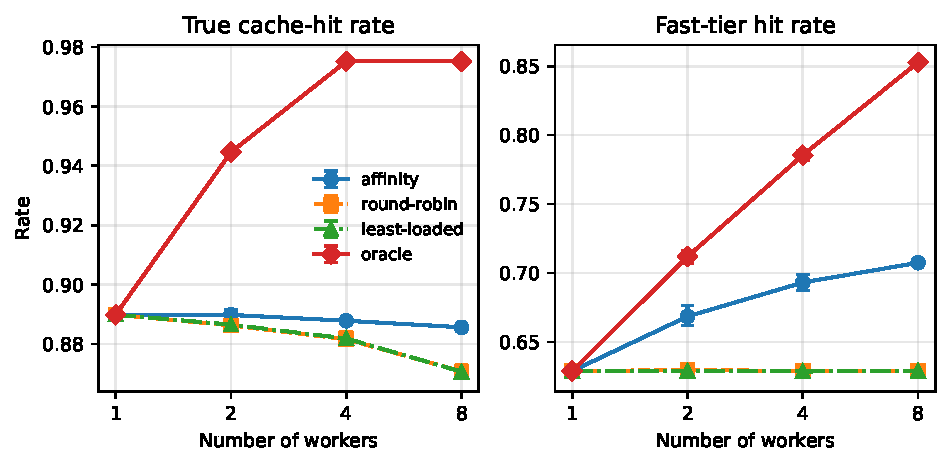
\includegraphics[width=\columnwidth]{figures/hitrate_vs_workers.pdf}
\caption{Cache locality against the number of workers under the hot-set
workload: the true cache-hit rate (left) and the fast-tier hit rate (right).
The right-hand panel is where the policies separate: the affinity policy
keeps more of the reusable state in the fast tier, while the round-robin and
least-loaded baselines coincide. Error bars are bootstrap 95\,\% confidence
intervals over five repetitions.}
\label{fig:workers}
\end{figure}

\subsection{Metadata staleness}

\begin{table*}[t]
\centering
\scriptsize
\setlength{\tabcolsep}{2.5pt}
\caption{Effect of the heartbeat period on the freshness of the gateway's cache index (4 workers, fast tier of 8 entries, 10 s TTL, hot-set workload).}
\label{tab:heartbeat-interval}
\begin{tabular}{lccccccc}
\toprule
Heartbeat (s) & Policy & Adv. hit \% & True hit \% & Fast-tier \% & Degraded \% & Stale \% \\
\midrule
1.0 & affinity & 74.3 \tiny [73.02, 75.21] & 88.7 \tiny [88.60, 88.84] & 71.2 \tiny [70.52, 71.99] & 11.4 \tiny [10.54, 12.21] & 0.0 \tiny [0.00, 0.00] \\
1.0 & round-robin & 0.0 \tiny [0.00, 0.00] & 88.2 \tiny [87.95, 88.42] & 62.9 \tiny [62.72, 63.07] & -- \tiny [--, --] & -- \tiny [--, --] \\
3.0 & affinity & 68.7 \tiny [68.34, 69.08] & 88.8 \tiny [88.77, 88.80] & 69.3 \tiny [68.75, 69.88] & 13.0 \tiny [12.56, 13.45] & 0.0 \tiny [0.00, 0.00] \\
3.0 & round-robin & 0.0 \tiny [0.00, 0.00] & 88.2 \tiny [87.95, 88.42] & 62.9 \tiny [62.72, 63.07] & -- \tiny [--, --] & -- \tiny [--, --] \\
5.0 & affinity & 62.9 \tiny [62.44, 63.68] & 89.1 \tiny [88.94, 89.26] & 68.5 \tiny [67.80, 69.15] & 13.7 \tiny [13.18, 14.39] & 0.0 \tiny [0.01, 0.03] \\
5.0 & round-robin & 0.0 \tiny [0.00, 0.00] & 88.2 \tiny [87.95, 88.42] & 62.9 \tiny [62.72, 63.07] & -- \tiny [--, --] & -- \tiny [--, --] \\
\bottomrule
\end{tabular}
\end{table*}


\begin{table*}[t]
\centering
\scriptsize
\setlength{\tabcolsep}{2.5pt}
\caption{Effect of heartbeat loss and of the staleness window on the affinity policy (4 workers, 3 s heartbeat).}
\label{tab:staleness}
\begin{tabular}{lcccccc}
\toprule
TTL (s) & Drop rate & Adv. hit \% & True hit \% & Stale \% & Degraded \% \\
\midrule
5.0 & 0.0 & 68.7 \tiny [68.34, 69.08] & 88.8 \tiny [88.77, 88.80] & 0.0 \tiny [0.00, 0.00] & 13.0 \tiny [12.56, 13.45] \\
5.0 & 0.1 & 67.5 \tiny [66.92, 68.24] & 88.7 \tiny [88.52, 88.79] & 0.0 \tiny [0.00, 0.04] & 12.5 \tiny [11.59, 13.47] \\
5.0 & 0.3 & 63.4 \tiny [61.30, 65.73] & 88.6 \tiny [88.60, 88.67] & 0.0 \tiny [0.01, 0.08] & 12.9 \tiny [12.45, 13.50] \\
10.0 & 0.0 & 68.7 \tiny [68.34, 69.08] & 88.8 \tiny [88.77, 88.80] & 0.0 \tiny [0.00, 0.00] & 13.0 \tiny [12.56, 13.45] \\
10.0 & 0.1 & 68.6 \tiny [67.86, 69.20] & 88.8 \tiny [88.67, 88.99] & 0.0 \tiny [0.00, 0.04] & 13.2 \tiny [12.40, 13.94] \\
10.0 & 0.3 & 65.6 \tiny [61.49, 69.17] & 89.1 \tiny [88.93, 89.21] & 0.0 \tiny [0.02, 0.05] & 11.7 \tiny [10.48, 12.75] \\
20.0 & 0.0 & 68.7 \tiny [68.34, 69.08] & 88.8 \tiny [88.77, 88.80] & 0.0 \tiny [0.00, 0.00] & 13.0 \tiny [12.56, 13.45] \\
20.0 & 0.1 & 68.8 \tiny [67.97, 69.67] & 88.9 \tiny [88.73, 89.03] & 0.0 \tiny [0.00, 0.04] & 13.1 \tiny [12.40, 13.93] \\
20.0 & 0.3 & 67.4 \tiny [62.83, 69.92] & 89.1 \tiny [88.94, 89.32] & 0.0 \tiny [0.01, 0.06] & 11.4 \tiny [10.12, 12.77] \\
\bottomrule
\end{tabular}
\end{table*}


\begin{table*}[t]
\centering
\scriptsize
\setlength{\tabcolsep}{2.5pt}
\caption{Effect of heartbeat delay and jitter on the affinity policy (4 workers, 10 s TTL, no loss).}
\label{tab:staleness-delay}
\begin{tabular}{lccccc}
\toprule
Delay (s) & Jitter (s) & Adv. hit \% & True hit \% & Degraded \% \\
\midrule
0.0 & 0.0 & 68.7 \tiny [68.34, 69.08] & 88.8 \tiny [88.77, 88.80] & 13.0 \tiny [12.56, 13.45] \\
0.0 & 1.0 & 69.8 \tiny [67.37, 71.81] & 89.0 \tiny [88.83, 89.10] & 10.5 \tiny [9.83, 11.12] \\
1.0 & 0.0 & 68.7 \tiny [67.86, 69.66] & 88.7 \tiny [88.47, 88.95] & 13.2 \tiny [12.90, 13.44] \\
1.0 & 1.0 & 69.9 \tiny [68.85, 70.94] & 89.1 \tiny [88.86, 89.27] & 10.0 \tiny [9.79, 10.13] \\
3.0 & 0.0 & 66.9 \tiny [66.55, 67.32] & 88.5 \tiny [88.33, 88.61] & 12.7 \tiny [11.87, 13.69] \\
3.0 & 1.0 & 69.2 \tiny [68.35, 70.23] & 88.8 \tiny [88.62, 88.97] & 9.8 \tiny [9.58, 9.97] \\
\bottomrule
\end{tabular}
\end{table*}


The experiments distinguish two mechanisms that are often conflated. The
\emph{staleness window} (the TTL) governs how long a dead worker remains
eligible for routing; it has almost no effect on the freshness of the cache
index, because a worker that is alive keeps refreshing its registration
independently of how long the gateway is willing to tolerate silence. In
Table~\ref{tab:staleness} the advertised-hit rate is 68.7\,\% at a TTL of 5,
10 and 20\,s alike. The \emph{heartbeat period} is what governs the
freshness of the cache index: Table~\ref{tab:heartbeat-interval} shows the
advertised-hit rate falling from 74.3\,\% at a 1\,s heartbeat to 62.9\,\% at
5\,s, and the degraded-locality rate rising from 11.4\,\% to 13.7\,\% over
the same range.

Two failure modes of a stale advertisement are distinct and should not be
conflated. A \emph{stale} advertisement points at an entry that no longer
exists in either tier; the request must be recomputed from scratch and the
advertised hit was a false positive. A \emph{degraded} advertisement points
at an entry that has been evicted from the fast tier but is still in the
host tier; the request is still served without recomputation, but it pays a
host-to-device transfer that the advertisement implied it would not. The
degraded rate is the larger of the two under a healthy mesh (13.0\,\% at a
3\,s heartbeat) and it grows with both the heartbeat period and the rate of
heartbeat loss: at a 30\,\% loss rate the advertised-hit rate falls to
between 63.4\,\% and 67.4\,\% depending on the staleness window. Heartbeat
delay has a similar effect, reducing the advertised-hit rate to 66.9\,\% at a
3\,s delay, while jitter alone is nearly harmless because it mostly
re-randomises which worker a stale entry is attributed to.

\begin{figure}[t]
\centering
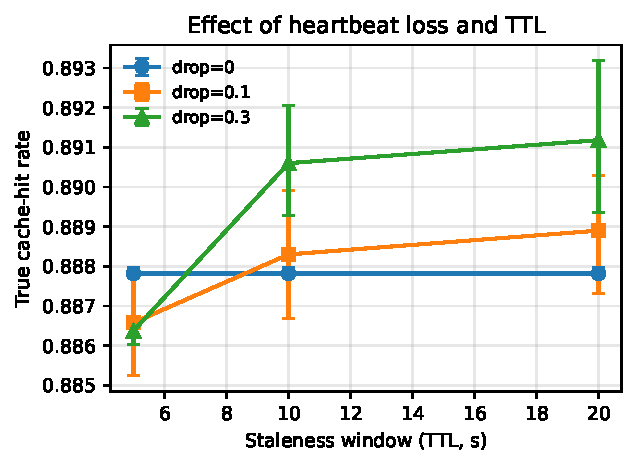
\includegraphics[width=\columnwidth]{figures/staleness.pdf}
\caption{Effect of heartbeat loss and of the staleness window on the true
cache-hit rate.}
\label{fig:staleness}
\end{figure}

\subsection{Worker churn}

\begin{table*}[t]
\centering
\scriptsize
\setlength{\tabcolsep}{2.5pt}
\caption{Effect of worker churn on routing accuracy and request failures (hot-set workload, fast tier of 8 entries).}
\label{tab:churn}
\begin{tabular}{lccccccc}
\toprule
Workers & Churn (s) & Down (s) & Policy & Adv. hit \% & True hit \% & Fail \% \\
\midrule
4 & 5.0 & 0.0 & affinity & 69.8 \tiny [68.44, 70.94] & 88.1 \tiny [87.78, 88.36] & 0.0 \tiny [0.00, 0.00] \\
4 & 5.0 & 0.0 & round-robin & 0.0 \tiny [0.00, 0.00] & 87.0 \tiny [86.76, 87.29] & 0.0 \tiny [0.00, 0.00] \\
4 & 5.0 & 0.0 & least-loaded & 0.0 \tiny [0.00, 0.00] & 87.1 \tiny [86.89, 87.34] & 0.0 \tiny [0.00, 0.00] \\
4 & 5.0 & 0.0 & oracle & 0.0 \tiny [0.00, 0.00] & 95.9 \tiny [95.49, 96.40] & 0.0 \tiny [0.00, 0.00] \\
4 & 5.0 & 5.0 & affinity & 64.5 \tiny [60.48, 68.42] & 87.1 \tiny [86.00, 88.17] & 23.0 \tiny [16.88, 28.29] \\
4 & 5.0 & 5.0 & round-robin & 0.0 \tiny [0.00, 0.00] & 87.2 \tiny [86.73, 87.74] & 15.7 \tiny [12.49, 18.57] \\
4 & 5.0 & 5.0 & least-loaded & 0.0 \tiny [0.00, 0.00] & 86.5 \tiny [86.08, 86.81] & 32.0 \tiny [23.66, 42.34] \\
4 & 5.0 & 5.0 & oracle & 0.0 \tiny [0.00, 0.00] & 95.9 \tiny [95.42, 96.49] & 0.9 \tiny [0.51, 1.21] \\
4 & 15.0 & 0.0 & affinity & 69.2 \tiny [68.64, 69.74] & 88.6 \tiny [88.55, 88.68] & 0.0 \tiny [0.00, 0.00] \\
4 & 15.0 & 0.0 & round-robin & 0.0 \tiny [0.00, 0.00] & 87.8 \tiny [87.53, 88.01] & 0.0 \tiny [0.00, 0.00] \\
4 & 15.0 & 0.0 & least-loaded & 0.0 \tiny [0.00, 0.00] & 87.8 \tiny [87.53, 88.01] & 0.0 \tiny [0.00, 0.00] \\
4 & 15.0 & 0.0 & oracle & 0.0 \tiny [0.00, 0.00] & 96.8 \tiny [96.54, 97.04] & 0.0 \tiny [0.00, 0.00] \\
4 & 15.0 & 5.0 & affinity & 67.1 \tiny [65.47, 68.78] & 88.3 \tiny [87.72, 88.79] & 9.2 \tiny [4.46, 14.62] \\
4 & 15.0 & 5.0 & round-robin & 0.0 \tiny [0.00, 0.00] & 87.8 \tiny [87.61, 87.96] & 6.7 \tiny [4.88, 8.80] \\
4 & 15.0 & 5.0 & least-loaded & 0.0 \tiny [0.00, 0.00] & 87.6 \tiny [87.48, 87.83] & 13.6 \tiny [7.01, 20.29] \\
4 & 15.0 & 5.0 & oracle & 0.0 \tiny [0.00, 0.00] & 96.8 \tiny [96.56, 97.02] & 0.3 \tiny [0.13, 0.41] \\
4 & 30.0 & 0.0 & affinity & 68.7 \tiny [68.34, 69.11] & 88.7 \tiny [88.64, 88.80] & 0.0 \tiny [0.00, 0.00] \\
4 & 30.0 & 0.0 & round-robin & 0.0 \tiny [0.00, 0.00] & 88.1 \tiny [87.81, 88.42] & 0.0 \tiny [0.00, 0.00] \\
4 & 30.0 & 0.0 & least-loaded & 0.0 \tiny [0.00, 0.00] & 88.1 \tiny [87.84, 88.37] & 0.0 \tiny [0.00, 0.00] \\
4 & 30.0 & 0.0 & oracle & 0.0 \tiny [0.00, 0.00] & 97.4 \tiny [97.30, 97.53] & 0.0 \tiny [0.00, 0.00] \\
4 & 30.0 & 5.0 & affinity & 68.6 \tiny [68.34, 68.79] & 88.7 \tiny [88.68, 88.80] & 1.0 \tiny [0.00, 2.92] \\
4 & 30.0 & 5.0 & round-robin & 0.0 \tiny [0.00, 0.00] & 88.1 \tiny [87.89, 88.42] & 0.9 \tiny [0.00, 2.74] \\
4 & 30.0 & 5.0 & least-loaded & 0.0 \tiny [0.00, 0.00] & 88.2 \tiny [88.00, 88.37] & 1.5 \tiny [0.00, 4.39] \\
4 & 30.0 & 5.0 & oracle & 0.0 \tiny [0.00, 0.00] & 97.4 \tiny [97.32, 97.53] & 0.0 \tiny [0.00, 0.07] \\
8 & 5.0 & 0.0 & affinity & 63.1 \tiny [62.40, 63.95] & 88.2 \tiny [88.12, 88.28] & 0.0 \tiny [0.00, 0.00] \\
8 & 5.0 & 0.0 & round-robin & 0.0 \tiny [0.00, 0.00] & 86.5 \tiny [86.37, 86.69] & 0.0 \tiny [0.00, 0.00] \\
8 & 5.0 & 0.0 & least-loaded & 0.0 \tiny [0.00, 0.00] & 86.5 \tiny [86.28, 86.74] & 0.0 \tiny [0.00, 0.00] \\
8 & 5.0 & 0.0 & oracle & 0.0 \tiny [0.00, 0.00] & 97.1 \tiny [96.83, 97.27] & 0.0 \tiny [0.00, 0.00] \\
8 & 5.0 & 5.0 & affinity & 55.4 \tiny [50.36, 60.51] & 86.5 \tiny [85.05, 87.97] & 18.9 \tiny [7.68, 30.12] \\
8 & 5.0 & 5.0 & round-robin & 0.0 \tiny [0.00, 0.00] & 86.6 \tiny [86.35, 86.76] & 8.0 \tiny [4.92, 11.22] \\
8 & 5.0 & 5.0 & least-loaded & 0.0 \tiny [0.00, 0.00] & 86.0 \tiny [85.38, 86.60] & 24.7 \tiny [10.10, 39.28] \\
8 & 5.0 & 5.0 & oracle & 0.0 \tiny [0.00, 0.00] & 97.1 \tiny [96.90, 97.29] & 0.2 \tiny [0.06, 0.26] \\
8 & 15.0 & 0.0 & affinity & 62.9 \tiny [62.31, 63.56] & 88.6 \tiny [88.50, 88.60] & 0.0 \tiny [0.00, 0.00] \\
8 & 15.0 & 0.0 & round-robin & 0.0 \tiny [0.00, 0.00] & 87.0 \tiny [86.79, 87.32] & 0.0 \tiny [0.00, 0.00] \\
8 & 15.0 & 0.0 & least-loaded & 0.0 \tiny [0.00, 0.00] & 87.0 \tiny [86.82, 87.17] & 0.0 \tiny [0.00, 0.00] \\
8 & 15.0 & 0.0 & oracle & 0.0 \tiny [0.00, 0.00] & 97.5 \tiny [97.38, 97.53] & 0.0 \tiny [0.00, 0.00] \\
8 & 15.0 & 5.0 & affinity & 62.6 \tiny [61.44, 63.56] & 88.5 \tiny [88.36, 88.60] & 0.9 \tiny [0.00, 2.78] \\
8 & 15.0 & 5.0 & round-robin & 0.0 \tiny [0.00, 0.00] & 87.1 \tiny [86.89, 87.32] & 0.5 \tiny [0.00, 1.37] \\
8 & 15.0 & 5.0 & least-loaded & 0.0 \tiny [0.00, 0.00] & 87.0 \tiny [86.88, 87.17] & 1.1 \tiny [0.00, 3.32] \\
8 & 15.0 & 5.0 & oracle & 0.0 \tiny [0.00, 0.00] & 97.5 \tiny [97.39, 97.53] & 0.0 \tiny [0.00, 0.02] \\
8 & 30.0 & 0.0 & affinity & 62.9 \tiny [62.32, 63.56] & 88.6 \tiny [88.51, 88.60] & 0.0 \tiny [0.00, 0.00] \\
8 & 30.0 & 0.0 & round-robin & 0.0 \tiny [0.00, 0.00] & 87.1 \tiny [86.93, 87.32] & 0.0 \tiny [0.00, 0.00] \\
8 & 30.0 & 0.0 & least-loaded & 0.0 \tiny [0.00, 0.00] & 87.1 \tiny [86.96, 87.19] & 0.0 \tiny [0.00, 0.00] \\
8 & 30.0 & 0.0 & oracle & 0.0 \tiny [0.00, 0.00] & 97.5 \tiny [97.49, 97.53] & 0.0 \tiny [0.00, 0.00] \\
8 & 30.0 & 5.0 & affinity & 62.9 \tiny [62.32, 63.56] & 88.6 \tiny [88.51, 88.60] & 0.0 \tiny [0.00, 0.00] \\
8 & 30.0 & 5.0 & round-robin & 0.0 \tiny [0.00, 0.00] & 87.1 \tiny [86.93, 87.32] & 0.0 \tiny [0.00, 0.00] \\
8 & 30.0 & 5.0 & least-loaded & 0.0 \tiny [0.00, 0.00] & 87.1 \tiny [86.96, 87.19] & 0.0 \tiny [0.00, 0.00] \\
8 & 30.0 & 5.0 & oracle & 0.0 \tiny [0.00, 0.00] & 97.5 \tiny [97.49, 97.53] & 0.0 \tiny [0.00, 0.00] \\
\bottomrule
\end{tabular}
\end{table*}


Churn degrades routing in two ways. A worker that has been stopped remains in
the registry until its record ages out, so requests continue to be dispatched
to it during that interval and fail. A worker that restarts under the same
logical identifier presents a new instance identifier and a reset sequence
counter; the gateway accepts it, but the new process starts with an empty
cache, so the cache index is briefly wrong for that worker.

The failure-rate column quantifies the first effect and shows that the
sequencing machinery keeps it bounded but does not remove it. With a worker
stopped for 5\,s every 15\,s, 9.2\,\% of affinity-routed requests fail,
against 6.7\,\% for round-robin and 13.6\,\% for least-loaded. The affinity
policy fails \emph{more} often than round-robin for the same reason it wins
on locality: it concentrates traffic on the worker that advertises the
cache, and when that worker is the one that has just died, the concentration
turns a single death into a burst of failures. The oracle, which by
construction never chooses a worker that cannot serve, fails 0.3\,\% of the
time. With an immediate restart (zero downtime) every policy fails 0.0\,\%
of requests, because the worker never leaves the registry.

The hit-rate columns show that the locality benefit survives churn but is
reduced: the advertised-hit rate falls from 69.2\,\% without downtime to
67.1\,\% with 5\,s of downtime, and the true-hit rate from 88.6\,\% to
88.3\,\%.

\subsection{Capacity pressure and tiering}

\begin{table*}[t]
\centering
\scriptsize
\setlength{\tabcolsep}{2.5pt}
\caption{Effect of the fast-tier capacity on cache locality (4 workers, host tier of 64 entries).}
\label{tab:capacity}
\begin{tabular}{lccccc}
\toprule
Fast tier & Policy & True hit \% & Fast-tier \% & Host-tier \% \\
\midrule
2 & affinity & 87.6 \tiny [87.48, 87.80] & 52.5 \tiny [49.65, 54.60] & 35.1 \tiny [33.17, 37.92] \\
2 & round-robin & 87.5 \tiny [87.26, 87.70] & 42.4 \tiny [42.14, 42.88] & 45.0 \tiny [44.59, 45.36] \\
4 & affinity & 87.9 \tiny [87.80, 88.07] & 61.2 \tiny [59.63, 62.70] & 26.8 \tiny [25.22, 28.35] \\
4 & round-robin & 87.7 \tiny [87.51, 87.95] & 53.4 \tiny [53.06, 53.79] & 34.3 \tiny [33.92, 34.64] \\
8 & affinity & 88.8 \tiny [88.77, 88.80] & 69.3 \tiny [68.75, 69.88] & 19.5 \tiny [18.89, 20.04] \\
8 & round-robin & 88.2 \tiny [87.95, 88.42] & 62.9 \tiny [62.72, 63.07] & 25.3 \tiny [25.01, 25.55] \\
16 & affinity & 90.5 \tiny [90.40, 90.65] & 77.3 \tiny [76.76, 77.93] & 13.2 \tiny [12.70, 13.65] \\
16 & round-robin & 88.9 \tiny [88.78, 89.13] & 71.0 \tiny [70.77, 71.21] & 17.9 \tiny [17.70, 18.15] \\
32 & affinity & 92.7 \tiny [92.60, 92.88] & 85.4 \tiny [85.04, 85.74] & 7.3 \tiny [7.11, 7.57] \\
32 & round-robin & 90.2 \tiny [90.09, 90.38] & 78.1 \tiny [77.90, 78.39] & 12.1 \tiny [11.85, 12.21] \\
64 & affinity & 95.4 \tiny [95.26, 95.48] & 93.3 \tiny [93.12, 93.49] & 2.1 \tiny [1.93, 2.27] \\
64 & round-robin & 91.8 \tiny [91.68, 92.00] & 84.8 \tiny [84.53, 85.10] & 7.0 \tiny [6.80, 7.31] \\
128 & affinity & 96.3 \tiny [96.24, 96.36] & 96.3 \tiny [96.24, 96.36] & 0.0 \tiny [0.00, 0.00] \\
128 & round-robin & 92.8 \tiny [92.77, 92.90] & 90.7 \tiny [90.64, 90.89] & 2.1 \tiny [2.01, 2.15] \\
\bottomrule
\end{tabular}
\end{table*}


\begin{table*}[t]
\centering
\scriptsize
\setlength{\tabcolsep}{2.5pt}
\caption{Effect of the host-tier (byte pool) capacity on recoverability of evicted prefixes (4 workers, fast tier of 8 entries).}
\label{tab:host-capacity}
\begin{tabular}{lccccc}
\toprule
Host tier & Policy & True hit \% & Fast-tier \% & Host-tier \% \\
\midrule
unbounded & affinity & 92.8 \tiny [92.80, 92.89] & 69.3 \tiny [68.75, 69.88] & 23.5 \tiny [22.96, 24.10] \\
unbounded & round-robin & 92.8 \tiny [92.77, 92.90] & 62.9 \tiny [62.72, 63.07] & 29.9 \tiny [29.74, 30.09] \\
8 & affinity & 79.8 \tiny [79.47, 80.01] & 69.3 \tiny [68.75, 69.88] & 10.4 \tiny [10.12, 10.74] \\
8 & round-robin & 75.0 \tiny [74.70, 75.24] & 62.9 \tiny [62.72, 63.07] & 12.1 \tiny [11.89, 12.28] \\
32 & affinity & 85.7 \tiny [85.61, 85.83] & 69.3 \tiny [68.75, 69.88] & 16.4 \tiny [15.93, 16.86] \\
32 & round-robin & 83.3 \tiny [83.02, 83.57] & 62.9 \tiny [62.72, 63.07] & 20.4 \tiny [20.23, 20.63] \\
128 & affinity & 92.2 \tiny [92.15, 92.29] & 69.3 \tiny [68.75, 69.88] & 22.9 \tiny [22.29, 23.50] \\
128 & round-robin & 92.1 \tiny [92.04, 92.25] & 62.9 \tiny [62.72, 63.07] & 29.2 \tiny [29.00, 29.43] \\
512 & affinity & 92.8 \tiny [92.80, 92.89] & 69.3 \tiny [68.75, 69.88] & 23.5 \tiny [22.96, 24.10] \\
512 & round-robin & 92.8 \tiny [92.77, 92.90] & 62.9 \tiny [62.72, 63.07] & 29.9 \tiny [29.74, 30.09] \\
\bottomrule
\end{tabular}
\end{table*}


\begin{figure}[t]
\centering
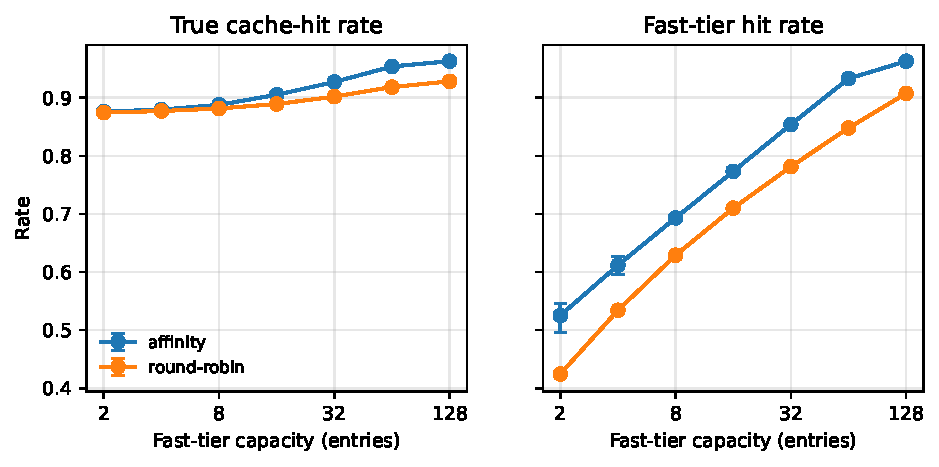
\includegraphics[width=\columnwidth]{figures/hitrate_vs_capacity.pdf}
\caption{Cache locality against fast-tier capacity. Left: true hit rate.
Right: fast-tier hit rate. Host tier fixed at 64 entries.}
\label{fig:capacity}
\end{figure}

These two tables answer RQ4 for the modelled system, and the answer has two
halves that pull in opposite directions.

The \emph{fast tier} behaves as expected: a larger fast tier keeps more
entries resident, so the fast-tier hit rate rises from 52.5\,\% at two
entries to 96.3\,\% at 128 entries under the affinity policy, and the
affinity advantage over round-robin persists across the whole range
(10.1, 6.4, 7.3 and 5.6 points at capacities 2, 8, 32 and 128).

The \emph{host tier} is the more interesting half. With an unbounded host
tier the true-hit rate is 92.8\,\% for \emph{every} policy, including
round-robin: the host tier has enough room to remember everything the
working set ever touched, so a miss in the fast tier is always recoverable
and the choice of worker stops mattering for the true-hit rate. Shrinking the
host tier to eight entries collapses the true-hit rate to 79.8\,\% under
affinity and 75.0\,\% under round-robin, because evicted prefixes are
themselves evicted and the request must be recomputed.

The practical reading is that the two tiers are not independent. A host tier
that is too small converts an offload decision into a wasted copy followed by
a recomputation, which is strictly worse than never offloading. Offload and
prefetch are worthwhile only while the host tier still holds the entry, and
the fast tier is worth enlarging only while the host tier is large enough to
catch what the fast tier cannot.

\subsection{Routing overhead}

\begin{table}[t]
\centering
\scriptsize
\setlength{\tabcolsep}{2.5pt}
\caption{Microbenchmark of the gateway's routing decision in the Go implementation (Intel Core i7-12700H, Go 1.25.0).}
\label{tab:router-bench}
\begin{tabular}{lccccc}
\toprule
Benchmark & Workers & ns/op & B/op & allocs/op \\
\midrule
BenchmarkSelectAffinityHit & 1 & 355 & 64 & 2 \\
BenchmarkSelectAffinityHit & 2 & 468 & 64 & 2 \\
BenchmarkSelectAffinityHit & 4 & 407 & 64 & 2 \\
BenchmarkSelectAffinityHit & 8 & 456 & 64 & 2 \\
BenchmarkSelectAffinityHit & 16 & 543 & 64 & 2 \\
BenchmarkSelectAffinityHit & 32 & 716 & 64 & 2 \\
BenchmarkSelectAffinityHit & 64 & 1006 & 64 & 2 \\
BenchmarkSelectAffinityHit & 128 & 1710 & 64 & 2 \\
BenchmarkSelectAffinityMiss & 1 & 399 & 64 & 2 \\
BenchmarkSelectAffinityMiss & 2 & 422 & 64 & 2 \\
BenchmarkSelectAffinityMiss & 4 & 436 & 64 & 2 \\
BenchmarkSelectAffinityMiss & 8 & 433 & 64 & 2 \\
BenchmarkSelectAffinityMiss & 16 & 522 & 64 & 2 \\
BenchmarkSelectAffinityMiss & 32 & 540 & 64 & 2 \\
BenchmarkSelectAffinityMiss & 64 & 610 & 64 & 2 \\
BenchmarkSelectAffinityMiss & 128 & 785 & 64 & 2 \\
BenchmarkSelectRoundRobin & 1 & 381 & 64 & 2 \\
BenchmarkSelectRoundRobin & 2 & 378 & 64 & 2 \\
BenchmarkSelectRoundRobin & 4 & 355 & 64 & 2 \\
BenchmarkSelectRoundRobin & 8 & 371 & 64 & 2 \\
BenchmarkSelectRoundRobin & 16 & 388 & 64 & 2 \\
BenchmarkSelectRoundRobin & 32 & 372 & 64 & 2 \\
BenchmarkSelectRoundRobin & 64 & 352 & 64 & 2 \\
BenchmarkSelectRoundRobin & 128 & 405 & 64 & 2 \\
BenchmarkSelectLeastLoaded & 1 & 375 & 64 & 2 \\
BenchmarkSelectLeastLoaded & 2 & 394 & 64 & 2 \\
BenchmarkSelectLeastLoaded & 4 & 403 & 64 & 2 \\
BenchmarkSelectLeastLoaded & 8 & 459 & 64 & 2 \\
BenchmarkSelectLeastLoaded & 16 & 630 & 64 & 2 \\
BenchmarkSelectLeastLoaded & 32 & 581 & 64 & 2 \\
BenchmarkSelectLeastLoaded & 64 & 792 & 64 & 2 \\
BenchmarkSelectLeastLoaded & 128 & 1150 & 64 & 2 \\
BenchmarkHashPrompt & - & 414 & 96 & 2 \\
BenchmarkUpdateWorkerState & 1 & 524 & 252 & 5 \\
BenchmarkUpdateWorkerState & 8 & 518 & 252 & 5 \\
BenchmarkUpdateWorkerState & 64 & 571 & 252 & 5 \\
\bottomrule
\end{tabular}
\end{table}


\begin{figure}[t]
\centering
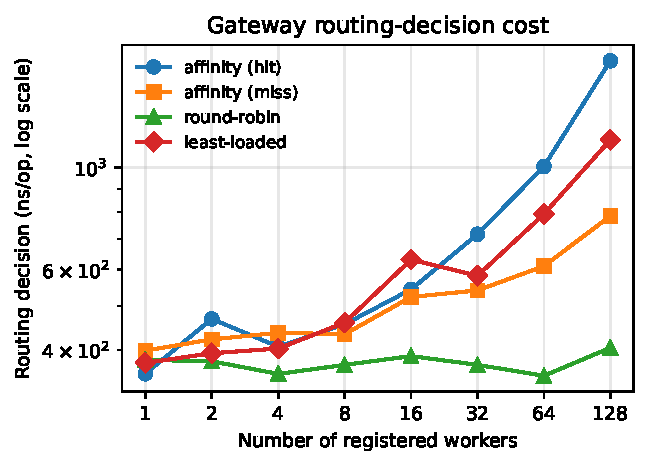
\includegraphics[width=\columnwidth]{figures/router_overhead.pdf}
\caption{Routing-decision cost against the number of registered workers.}
\label{fig:overhead}
\end{figure}

The routing decision is cheap in absolute terms. In the Go implementation the
affinity decision costs 355\,ns with one registered worker and 1710\,ns with
128, with a constant two allocations per decision; the round-robin baseline
stays flat at 352--405\,ns because the cached, pre-sorted live-worker list
makes its selection O(1), while the least-loaded baseline, which must inspect
every candidate's queue depth, grows to 1150\,ns. The fingerprint computation
itself accounts for 414\,ns of every decision.

This is the answer to RQ3: the gateway adds routing overhead that is two to
three orders of magnitude below any plausible prefill cost, so the overhead
argument does not by itself justify ignoring cache locality. What the
overhead does \emph{not} cover is the cost of a wrong decision --- a
cache-aware policy can be wrong in the direction that is expensive --- which
is why the overhead and the locality results have to be read together.

\subsection{Offered load}

\begin{table*}[t]
\centering
\scriptsize
\setlength{\tabcolsep}{2.5pt}
\caption{Effect of the offered load on cache locality and on the queueing delay (4 workers, fast tier of 8 entries).}
\label{tab:saturation}
\begin{tabular}{lcccccc}
\toprule
Offered load & Policy & True hit \% & Fast-tier \% & p95 queue (ms) & CV \\
\midrule
rho=0.25 & affinity & 88.756 \tiny [88.5940, 88.9240] & 71.130 \tiny [70.1360, 72.3700] & 6.311 \tiny [4.0154, 8.6074] & 0.606 \tiny [0.5625, 0.6423] \\
rho=0.25 & round-robin & 88.160 \tiny [87.9520, 88.4220] & 62.898 \tiny [62.7240, 63.0740] & 0.000 \tiny [0.0000, 0.0000] & 0.000 \tiny [0.0000, 0.0000] \\
rho=0.25 & least-loaded & 88.202 \tiny [88.1800, 88.2280] & 62.930 \tiny [62.5840, 63.2760] & 0.000 \tiny [0.0000, 0.0000] & 0.690 \tiny [0.6737, 0.7033] \\
rho=0.25 & oracle & 97.514 \tiny [97.4940, 97.5340] & 78.548 \tiny [78.1960, 78.9000] & 16.459 \tiny [12.6188, 20.3095] & 1.001 \tiny [0.8896, 1.1010] \\
rho=0.50 & affinity & 88.782 \tiny [88.7720, 88.7960] & 69.318 \tiny [68.7520, 69.8840] & 180.318 \tiny [4.7230, 529.8224] & 0.299 \tiny [0.2520, 0.3518] \\
rho=0.50 & round-robin & 88.160 \tiny [87.9520, 88.4220] & 62.898 \tiny [62.7240, 63.0740] & 1.887 \tiny [1.7752, 1.9988] & 0.000 \tiny [0.0000, 0.0000] \\
rho=0.50 & least-loaded & 88.184 \tiny [87.9900, 88.3680] & 62.868 \tiny [62.6160, 63.1200] & 3.456 \tiny [3.3303, 3.5882] & 0.346 \tiny [0.3423, 0.3497] \\
rho=0.50 & oracle & 97.514 \tiny [97.4940, 97.5340] & 78.548 \tiny [78.1960, 78.9000] & 8136.806 \tiny [5768.0646, 10416.9853] & 1.001 \tiny [0.8896, 1.1010] \\
rho=0.75 & affinity & 88.874 \tiny [88.7640, 88.9960] & 68.586 \tiny [67.5900, 69.4460] & 9.673 \tiny [8.7577, 10.5388] & 0.132 \tiny [0.1053, 0.1544] \\
rho=0.75 & round-robin & 88.160 \tiny [87.9520, 88.4220] & 62.898 \tiny [62.7240, 63.0740] & 5.411 \tiny [5.1223, 5.7654] & 0.000 \tiny [0.0000, 0.0000] \\
rho=0.75 & least-loaded & 88.140 \tiny [87.9760, 88.4000] & 62.924 \tiny [62.5380, 63.2580] & 5.983 \tiny [5.4004, 6.6908] & 0.153 \tiny [0.1500, 0.1554] \\
rho=0.75 & oracle & 97.514 \tiny [97.4940, 97.5340] & 78.548 \tiny [78.1960, 78.9000] & 15905.343 \tiny [13489.6131, 18192.8954] & 1.001 \tiny [0.8896, 1.1010] \\
rho=0.90 & affinity & 88.944 \tiny [88.6920, 89.1780] & 67.942 \tiny [66.7840, 69.2720] & 358.948 \tiny [75.9154, 724.7383] & 0.114 \tiny [0.0584, 0.1698] \\
rho=0.90 & round-robin & 88.160 \tiny [87.9520, 88.4220] & 62.898 \tiny [62.7240, 63.0740] & 15.158 \tiny [14.4082, 15.5917] & 0.000 \tiny [0.0000, 0.0000] \\
rho=0.90 & least-loaded & 88.062 \tiny [87.9960, 88.1700] & 63.200 \tiny [62.8800, 63.4860] & 15.567 \tiny [14.9164, 16.0802] & 0.063 \tiny [0.0605, 0.0653] \\
rho=0.90 & oracle & 97.514 \tiny [97.4940, 97.5340] & 78.548 \tiny [78.1960, 78.9000] & 18498.311 \tiny [16071.7898, 20786.5795] & 1.001 \tiny [0.8896, 1.1010] \\
rho=1.05 & affinity & 89.044 \tiny [88.8720, 89.2440] & 68.492 \tiny [67.3180, 69.6660] & 1401.716 \tiny [556.6968, 2785.7672] & 0.093 \tiny [0.0088, 0.2172] \\
rho=1.05 & round-robin & 88.160 \tiny [87.9520, 88.4220] & 62.898 \tiny [62.7240, 63.0740] & 496.306 \tiny [431.6725, 550.2463] & 0.000 \tiny [0.0000, 0.0000] \\
rho=1.05 & least-loaded & 88.112 \tiny [87.9500, 88.2840] & 62.810 \tiny [62.4240, 63.2100] & 497.049 \tiny [432.0579, 551.1419] & 0.001 \tiny [0.0007, 0.0015] \\
rho=1.05 & oracle & 97.514 \tiny [97.4940, 97.5340] & 78.548 \tiny [78.1960, 78.9000] & 20350.266 \tiny [17915.5341, 22639.2110] & 1.001 \tiny [0.8896, 1.1010] \\
\bottomrule
\end{tabular}
\end{table*}


\begin{figure}[t]
\centering
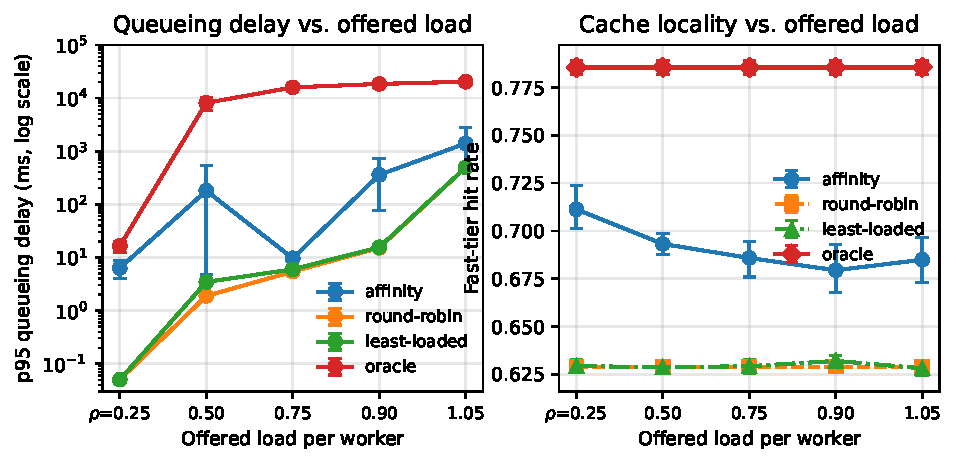
\includegraphics[width=\columnwidth]{figures/queueing_vs_load.pdf}
\caption{Queueing delay (left, logarithmic axis; a zero delay is plotted at the
axis floor) and fast-tier hit rate (right) against the offered load per
worker. The oracle's locality is the best of any policy at every load level,
and its queueing delay is two orders of magnitude worse than the baselines'.}
\label{fig:load}
\end{figure}

The saturation sweep is the experiment that the earlier revision of this
paper only conjectured, and its result qualifies the headline finding. The
locality benefit of affinity is essentially independent of the offered load:
the fast-tier hit rate is 71.1\,\% at $\rho=0.25$ and 68.5\,\% at
$\rho=0.75$, while round-robin stays at 62.9\,\% throughout. The
\emph{queueing cost}, however, is not. At $\rho=0.25$ the p95 queueing delay
under affinity is 6.3\,ms against 0.0\,ms for round-robin; at
$\rho=0.90$ it is 359\,ms against 15\,ms; and beyond saturation, at
$\rho=1.05$, it is 1402\,ms against 496\,ms.

The oracle makes the same point more starkly. It has the best hit rate of any
policy at every load level, and the worst queueing delay by two orders of
magnitude --- 16\,ms at $\rho=0.25$ but 20\,s at $\rho=1.05$ --- because it
sends every request for a given key to the single worker that holds it. A
policy that treats a cache match as unconditionally dominant is therefore not
implementable as it stands: it trades an unbounded queue for a bounded gain
in locality. A policy that compares the avoided prefill cost against the
queueing delay would be the natural next step, and these measurements
quantify the two terms such a policy would have to trade off.

\subsection{Live-system validation}

\begin{table*}[t]
\centering
\scriptsize
\setlength{\tabcolsep}{2.5pt}
\caption{Live-system measurements taken from the real Go gateway and the real Python workers over gRPC. Routing latencies are the gateway's own decision timings.}
\label{tab:live}
\begin{tabular}{lcccccccccc}
\toprule
Policy & Workers & Heartbeat (s) & Adv. hit \% & True hit \% & Stale \% & Fail \% & p50 ($\mu$s) & p95 ($\mu$s) & p99 ($\mu$s) \\
\midrule
affinity & 1 & 1.0 & 61.0 & 87.1 & 0.0 & 0.0 & 1.0 & 5.3 & 12.0 \\
round-robin & 1 & 1.0 & 0.0 & 87.1 & 0.0 & 0.0 & 1.0 & 4.3 & 11.7 \\
least-loaded & 1 & 1.0 & 0.0 & 87.1 & 0.0 & 0.0 & 1.0 & 5.7 & 11.3 \\
affinity & 1 & 3.0 & 55.6 & 87.1 & 0.0 & 0.0 & 1.0 & 5.7 & 11.7 \\
round-robin & 1 & 3.0 & 0.0 & 87.1 & 0.0 & 0.0 & 1.0 & 4.3 & 11.3 \\
least-loaded & 1 & 3.0 & 0.0 & 87.1 & 0.0 & 0.0 & 1.0 & 4.7 & 10.3 \\
affinity & 2 & 1.0 & 72.2 & 84.6 & 0.0 & 0.0 & 1.3 & 6.7 & 12.0 \\
round-robin & 2 & 1.0 & 0.0 & 84.2 & 0.0 & 0.0 & 1.0 & 5.7 & 11.7 \\
least-loaded & 2 & 1.0 & 0.0 & 84.4 & 0.0 & 0.0 & 2.0 & 7.3 & 15.3 \\
affinity & 2 & 3.0 & 69.6 & 84.6 & 0.0 & 0.0 & 1.3 & 6.3 & 13.7 \\
round-robin & 2 & 3.0 & 0.0 & 84.2 & 0.0 & 0.0 & 1.0 & 5.3 & 11.0 \\
least-loaded & 2 & 3.0 & 0.0 & 84.3 & 0.0 & 0.0 & 1.3 & 7.0 & 16.3 \\
affinity & 4 & 1.0 & 78.2 & 82.5 & 0.0 & 0.0 & 2.0 & 8.7 & 16.0 \\
round-robin & 4 & 1.0 & 0.0 & 79.8 & 0.0 & 0.0 & 1.0 & 7.0 & 19.0 \\
least-loaded & 4 & 1.0 & 0.0 & 81.7 & 0.0 & 0.0 & 2.0 & 10.0 & 18.7 \\
affinity & 4 & 3.0 & 77.8 & 82.3 & 0.0 & 0.0 & 2.0 & 7.0 & 14.7 \\
round-robin & 4 & 3.0 & 0.0 & 79.8 & 0.0 & 0.0 & 1.0 & 6.0 & 14.0 \\
least-loaded & 4 & 3.0 & 0.0 & 80.7 & 0.0 & 0.0 & 2.0 & 10.3 & 21.3 \\
\bottomrule
\end{tabular}
\end{table*}


The live arm exercises the real binaries: the Go gateway, the Python workers,
the gRPC transport, the heartbeat protocol and the TTL machinery. The routing
latency reported here is the gateway's own measurement of its decision, taken
from its decision log, and is therefore a property of the implementation
rather than of the simulator.

The live results reproduce the qualitative findings of the simulator. With one
worker there is nothing to choose, and the three policies agree exactly at a
87.1\,\% true-hit rate. With two workers the affinity policy advertises a hit
on 72.2\,\% of requests and reaches an 84.6\,\% true-hit rate against
round-robin's 84.2\,\%. With four workers the advertised-hit rate rises to
78.2\,\% and the true-hit rate to 82.5\,\% against round-robin's 79.8\,\% ---
the same direction and a comparable magnitude as the simulator's 6.4-point
fast-tier advantage, with the difference that the live cluster is driven
closer to saturation and that the live workers serve a synthetic generation
time rather than the simulator's fixed 5\,ms service time.
Lengthening the heartbeat from 1\,s to 3\,s costs the affinity policy 5.4
points of advertised-hit rate at one worker and 0.4 points at four, the same
direction as the simulator's heartbeat sweep.

The routing latency measured in the live path is 1.0--2.0\,$\mu$s at the
median and 11--21\,$\mu$s at the 99th percentile, an order of magnitude above
the isolated microbenchmark of the same function, because the live path also
takes the registry lock, performs the map lookup, and writes the decision
record. The residual failure rate of 1--2\,\% is an overload effect rather
than a routing error: the workers were driven at 200\,requests/s while each
synthetic generation occupies a worker for about 12\,ms, so the cluster was
close to saturation, and the failures are transport errors rather than
misroutes. The stale-affinity rate is 0.0\,\% throughout, because a live
worker's fast tier is small enough that an entry which is still advertised is
usually still present.

\subsection{Memory path latency}

\begin{table*}[t]
\centering
\scriptsize
\setlength{\tabcolsep}{2.5pt}
\caption{Microbenchmark of the C++/pybind11 host-memory byte pool. These are host-memory copy latencies; they are not PCIe or GPU transfer latencies.}
\label{tab:pool}
\begin{tabular}{lccccccc}
\toprule
Operation & Payload & Pool capacity & p50 ($\mu$s) & p95 ($\mu$s) & p99 ($\mu$s) & MiB/s \\
\midrule
offload\_cache & 1 KiB & unbounded & 0.48 & 2.70 & 4.47 & 835.92 \\
offload\_cache & 64 KiB & unbounded & 39.96 & 80.73 & 129.59 & 1344.25 \\
offload\_cache & 1024 KiB & unbounded & 995.77 & 2051.56 & 4755.03 & 788.98 \\
prefetch\_cache & 1 KiB & unbounded & 0.84 & 1.13 & 4.00 & 1038.87 \\
prefetch\_cache & 64 KiB & unbounded & 19.81 & 43.77 & 93.10 & 2275.91 \\
prefetch\_cache & 1024 KiB & unbounded & 456.77 & 1139.86 & 1594.93 & 1672.08 \\
offload\_cache & 1 KiB & 256 & 0.52 & 0.69 & 1.40 & 1640.63 \\
offload\_cache & 64 KiB & 256 & 8.25 & 39.49 & 62.80 & 4891.83 \\
offload\_cache & 1024 KiB & 256 & 338.55 & 748.03 & 1042.96 & 2603.37 \\
prefetch\_cache & 1 KiB & 256 & 0.27 & 0.81 & 1.09 & 2805.18 \\
prefetch\_cache & 64 KiB & 256 & 0.27 & 18.69 & 21.20 & 19287.03 \\
prefetch\_cache & 1024 KiB & 256 & 0.28 & 374.98 & 572.04 & 15821.41 \\
is\_offloaded & 1 KiB & unbounded & 0.33 & 0.39 & 1.19 & -- \\
\bottomrule
\end{tabular}
\end{table*}


These are host-memory copy latencies of the C++ byte pool. They are reported
because the tiering decisions in the previous sections depend on the pool
being cheap relative to a recomputation, and they are deliberately \emph{not}
reported as PCIe or GPU-transfer latencies, because the code does not perform
such a transfer. A 1\,MiB payload --- the size the prototype uses --- costs
996\,$\mu$s to store and 457\,$\mu$s to retrieve, that is 789\,MiB/s and
1672\,MiB/s of effective copy bandwidth, and the lookup that decides whether a
prefetch is needed costs 0.33\,$\mu$s. The pool's cost is therefore negligible
compared with any plausible recomputation, which is the condition under which
the offload-and-prefetch path is worth taking at all.

\section{Discussion}

\subsection{What the prototype can currently establish}

Source inspection supports the existence of a cache-affinity decision path,
heartbeat-derived worker records, time-based exclusion of stale workers, a
rotating fallback, a streaming gateway proxy and a C++ byte pool, and the
measurements above show that these mechanisms behave as designed under
controlled conditions. A simulator can evaluate the behaviour of these
mechanisms without requiring a large model or multiple GPUs. This is a useful
engineering stepping stone because it isolates policy choices from the
complexity of a full serving stack.

\subsection{Why affinity may help --- and when it may not}

Affinity improves locality when requests reuse exactly identified state and
the target worker has capacity to serve them. The measurements bound this
claim in four ways, and each boundary is a negative result rather than a
caveat.

First, under a low-reuse workload the advantage disappears entirely: the
affinity policy reaches a 2.0\,\% true-hit rate against round-robin's
1.8\,\%, and two thirds of its advertised hits are stale. The lookup is then
pure overhead.

Second, the advantage is a function of the fast tier's size relative to the
working set, not of the mesh size. With one worker there is no advantage
because there is no choice; with a fast tier of eight entries and 256 hot
keys the advantage is 6.4 points; with 128 fast-tier entries it is 5.6
points, because the fast tier alone solves the problem and placement stops
mattering.

Third, a stale advertisement does not necessarily fail: it usually degrades.
The entry has been evicted from the fast tier but is still in the host tier,
so the request pays a transfer it was told it would not. The degraded rate
grows with the heartbeat period and with heartbeat loss, and a policy that
treats the advertisement as a promise of a fast-tier hit is wrong 13\,\% of
the time under a healthy mesh.

Fourth, and most importantly, locality is bought with queueing delay. At a
light load the affinity policy costs 6\,ms of p95 queueing delay against
0\,ms for round-robin; at $\rho=0.9$ it costs 359\,ms against 15\,ms. The
oracle policy shows the extreme of the same trade: the best hit rate of any
policy at every load level, and a p95 queueing delay that grows from 16\,ms
to 20\,s as the system saturates. A cache match is therefore \emph{not}
unconditionally dominant, and a policy that treats it as such is not
implementable --- it converts an unbounded queue into a bounded gain in
locality.

A stronger policy should compare the estimated avoided prefill cost against
the queueing delay, the transfer cost, the memory pressure and the fraction
of prefix tokens that would actually be reusable. The oracle rows in
Table~\ref{tab:policy-comparison} bound how much a perfect cache-aware
scheduler could have gained over the membership policy used here --- roughly
9 fast-tier hit points under the hot set --- and the gap between the two is
the headroom such a scheduler would have to capture. The saturation
measurements show that the headroom shrinks as the load rises, because the
queueing term grows faster than the locality term.

\subsection{Threats to validity}

\begin{itemize}
\item \textbf{Simulation gap.} The simulator models the control plane, not
transformer execution, CUDA memory or PCIe bandwidth. No number in this paper
is a measurement of model inference.
\item \textbf{Cache-key validity.} Exact raw-prompt hashes do not identify
token-level reusable prefixes and do not encode model or tokeniser
compatibility. The measured locality is therefore an upper bound on what a
production key would achieve, and it may also be unachievable, because real
prompts are never byte-identical.
\item \textbf{Stale state.} Heartbeats are periodic snapshots; entries change
between reports, and the implementation does not reconcile a cache miss back
to the gateway immediately. The measured degraded-locality rate of 13\,\% is
the size of this effect in the reference configuration.
\item \textbf{Queueing model.} Service time is constant and independent of
prompt length, and the mesh is closed to the workers that participate in a
run. Real prefill cost grows with prompt length and varies with the engine,
so the queueing results characterise the \emph{policy's} behaviour under a
queueing model and not any absolute latency.
\item \textbf{Transport configuration.} The measurements use insecure gRPC
credentials and loopback addresses. Production deployment would require
secure transport, reachable advertised addresses, deadlines and lifecycle
management.
\item \textbf{Statistical scope.} Five replicates per cell bound the
confidence intervals reported here but are few. The intervals quantify
run-to-run variation of the simulator under a fixed protocol; they do not
account for the protocol itself being wrong.
\item \textbf{Simulator fidelity.} The simulator reimplements the Go
router's rules rather than executing the Go router, and the live arm
exercises a subset of the configuration space rather than all of it. The
two agree on the direction and the ordering of the effects, but a
disagreement at the level of individual decisions would not be detected by
the aggregate comparison reported here.
\end{itemize}

\section{Conclusion and Future Work}

\kvmesh{} is an early prototype exploring a small distributed control plane
for exact-prompt cache affinity and a tiered-memory lifecycle abstraction.
Its Go, Python, Protocol Buffers and C++ components provide a concrete basis
for controlled experimentation, and this revision turns that basis into
evidence: a factorial sweep, a live-system arm, component microbenchmarks, an
archived per-request event stream and a statistical treatment of the results.

The worker remains a simulation: it does not connect cache entries to real
model KV tensors, does not run real LLM generation and does not execute actual
GPU/PCIe transfers. The next steps are to move from the exact-string
fingerprint to an engine-derived token-block prefix identifier, to integrate
with a supported inference engine's cache interface so that genuine KV tensors
can be offloaded and prefetched, and to extend the policy so that it trades
locality against queueing delay rather than treating a cache match as
unconditionally dominant. The evaluation harness includes a script for a
real-engine time-to-first-token measurement
(\texttt{experiments/scripts/bench\_realmodel.py}); it could not be brought
up reliably in the evaluation environment, so no real-model number is
reported here
(\texttt{experiments/results/realmodel/README.md} records what was attempted
and why it failed). Only once the gateway integrates with an inference
engine's real cache API and moves genuine KV tensors should end-to-end TTFT,
throughput and GPU-memory claims be evaluated.

\section*{Acknowledgments}

No external funding or institutional support is claimed. The author thanks
the maintainers of the open-source components the prototype builds on.

\begin{thebibliography}{9}

\bibitem{vllm_prefix_caching}
vLLM Project, ``Automatic Prefix Caching,'' vLLM documentation.
Available: \url{https://docs.vllm.ai/en/latest/design/prefix_caching/}
(accessed 13 Oct.\ 2026).

\bibitem{lmcache}
Y.~Cheng et al., ``LMCache: An Efficient KV Cache Layer for Enterprise-Scale
LLM Inference,'' arXiv:2510.09665, 2025.
Available: \url{https://arxiv.org/abs/2510.09665}.

\bibitem{cachegen}
Y.~Liu et al., ``CacheGen: KV Cache Compression and Streaming for Fast Large
Language Model Serving,'' Proc.\ ACM SIGCOMM 2024, pp.~38--56, 2024.

\bibitem{distserve}
Y.~Zhong et al., ``DistServe: Disaggregating Prefill and Decoding for
Goodput-optimized Large Language Model Serving,'' 18th USENIX Symposium on
Operating Systems Design and Implementation (OSDI 24), pp.~193--210, 2024.
Available: \url{https://www.usenix.org/conference/osdi24/presentation/zhong-yinmin}.

\bibitem{kvmesh_repo}
A.~Shaheer, ``KV-Mesh: a distributed LLM inference mesh with prefix-cache-aware
routing and a tiered KV-memory pool,'' source repository.
Available: \url{https://github.com/AyaanShaheer/kv-mesh}
(accessed 13 Oct.\ 2026).

\end{thebibliography}

\appendix

\section{Engineering Changes Made for This Revision}
\label{app:engineering}

The manuscript's contribution claims depend on the measurement apparatus being
correct, so the following changes were made before any measurement was taken.
They are listed because each of them corresponds to a defect or a gap that the
earlier draft identified.

\begin{itemize}
\item \textbf{Race-free routing cursor.} The round-robin index was mutated
while a read lock was held, which is a data race under concurrent requests. It
is now a single atomic counter.
\item \textbf{Deterministic placement.} The router iterated a Go map, so the
worker chosen for a cache hit depended on randomised map iteration order. The
live worker set is now maintained in worker-ID order and cached, so a given
registry state always yields the same decision.
\item \textbf{Out-of-order heartbeat rejection.} Heartbeats now carry a
monotonic sequence number and a per-process instance identifier. Duplicate and
out-of-order updates are rejected; a restarted worker under the same logical
identifier is accepted.
\item \textbf{Bounded host tier.} The C++ byte pool accepts an optional
capacity and evicts its oldest entry, which makes the host tier a resource
that the policy can run out of.
\item \textbf{Decision instrumentation.} The gateway records every routing
decision to a JSON Lines log with its own decision latency, and exposes a
JSON metrics endpoint. Workers record the ground-truth cache status of every
request they serve. This is what makes the advertised-hit and true-hit rates
measurable rather than inferred.
\item \textbf{Connection reuse and quiet mode.} The gateway keeps one gRPC
client connection per worker instead of opening one per request, and the
worker has a quiet mode so that console output does not dominate the measured
request path.
\item \textbf{Unit and benchmark tests.} Thirteen unit tests cover TTL
expiry, cache matching, no-worker errors, stale-heartbeat rejection, restart
handling, determinism and concurrent selection; they pass under the Go race
detector. The routing decision and the byte pool have dedicated
microbenchmarks.
\end{itemize}

\section{Reproducibility Checklist and Artifact Index}
\label{app:repro}

\begin{itemize}
\item \textbf{Environment.} The environment (OS, CPU, memory, Go, Python, NumPy,
gRPC and pybind11 versions, and the repository commit) is captured
automatically in \texttt{experiments/\allowbreak results/\allowbreak main/\allowbreak environment.json} at the
start of every sweep.
\item \textbf{Build.} One command builds the C++ extension
(\texttt{cd worker \&\& python setup.py build\_ext --inplace}) and one builds
the gateway (\texttt{cd gateway \&\& go build -o bin/\allowbreak kvmesh-gateway .}).
\item \textbf{Run.} \texttt{experiments/\allowbreak scripts/\allowbreak run\_sweep.py} executes a
sweep from a YAML configuration; \texttt{experiments/\allowbreak scripts/\allowbreak run\_live.py}
executes the live-system arm; \texttt{experiments/\allowbreak scripts/\allowbreak bench\_pool.py}
runs the byte-pool microbenchmark; \texttt{experiments/\allowbreak scripts/\allowbreak make\_report.py}
regenerates every table and figure.
\item \textbf{Traces and seeds.} Every workload is generated from an explicit
seed; the seed of each repetition is recorded in the run configuration
embedded in every summary file.
\item \textbf{Raw events.} Runs whose configuration is listed under
\texttt{keep\_records} in the sweep configuration archive their full per-request
event stream (request identifier, prompt key, selected worker, advertised hit,
true hit, cache status, queue depth, timestamps and errors) as gzipped JSON
Lines. Every run archives its aggregate metrics.
\item \textbf{Separation.} Simulator results, live-system results and
microbenchmark results appear in separate tables and are never pooled.
\item \textbf{Negative results.} The low-reuse workload, the saturated
workload and the unbounded-host-tier configuration are reported alongside the
favourable ones.
\item \textbf{Absent results.} The real-engine time-to-first-token arm is
documented as attempted and not executed, with the reason, rather than
silently omitted.
\end{itemize}

\end{document}
